%% bare_conf_compsoc.tex
%% V1.4b
%% 2015/08/26
%% by Michael Shell
%% See:
%% http://www.michaelshell.org/
%% for current contact information.
%%
%% This is a skeleton file demonstrating the use of IEEEtran.cls
%% (requires IEEEtran.cls version 1.8b or later) with an IEEE Computer
%% Society conference paper.
%%
%% Support sites:
%% http://www.michaelshell.org/tex/ieeetran/
%% http://www.ctan.org/pkg/ieeetran
%% and
%% http://www.ieee.org/

%%*************************************************************************
%% Legal Notice:
%% This code is offered as-is without any warranty either expressed or
%% implied; without even the implied warranty of MERCHANTABILITY or
%% FITNESS FOR A PARTICULAR PURPOSE!
%% User assumes all risk.
%% In no event shall the IEEE or any contributor to this code be liable for
%% any damages or losses, including, but not limited to, incidental,
%% consequential, or any other damages, resulting from the use or misuse
%% of any information contained here.
%%
%% All comments are the opinions of their respective authors and are not
%% necessarily endorsed by the IEEE.
%%
%% This work is distributed under the LaTeX Project Public License (LPPL)
%% ( http://www.latex-project.org/ ) version 1.3, and may be freely used,
%% distributed and modified. A copy of the LPPL, version 1.3, is included
%% in the base LaTeX documentation of all distributions of LaTeX released
%% 2003/12/01 or later.
%% Retain all contribution notices and credits.
%% ** Modified files should be clearly indicated as such, including  **
%% ** renaming them and changing author support contact information. **
%%*************************************************************************


% *** Authors should verify (and, if needed, correct) their LaTeX system  ***
% *** with the testflow diagnostic prior to trusting their LaTeX platform ***
% *** with production work. The IEEE's font choices and paper sizes can   ***
% *** trigger bugs that do not appear when using other class files.       ***                          ***
% The testflow support page is at:
% http://www.michaelshell.org/tex/testflow/



\documentclass[conference,compsoc]{IEEEtran}
% Some/most Computer Society conferences require the compsoc mode option,
% but others may want the standard conference format.
%
% If IEEEtran.cls has not been installed into the LaTeX system files,
% manually specify the path to it like:
% \documentclass[conference,compsoc]{../sty/IEEEtran}





% Some very useful LaTeX packages include:
% (uncomment the ones you want to load)


% *** MISC UTILITY PACKAGES ***
%
%\usepackage{ifpdf}
% Heiko Oberdiek's ifpdf.sty is very useful if you need conditional
% compilation based on whether the output is pdf or dvi.
% usage:
% \ifpdf
%   % pdf code
% \else
%   % dvi code
% \fi
% The latest version of ifpdf.sty can be obtained from:
% http://www.ctan.org/pkg/ifpdf
% Also, note that IEEEtran.cls V1.7 and later provides a builtin
% \ifCLASSINFOpdf conditional that works the same way.
% When switching from latex to pdflatex and vice-versa, the compiler may
% have to be run twice to clear warning/error messages.






% *** CITATION PACKAGES ***
%
\ifCLASSOPTIONcompsoc
  % IEEE Computer Society needs nocompress option
  % requires cite.sty v4.0 or later (November 2003)
  \usepackage[nocompress]{cite}
\else
  % normal IEEE
  \usepackage{cite}
\fi
% cite.sty was written by Donald Arseneau
% V1.6 and later of IEEEtran pre-defines the format of the cite.sty package
% \cite{} output to follow that of the IEEE. Loading the cite package will
% result in citation numbers being automatically sorted and properly
% "compressed/ranged". e.g., [1], [9], [2], [7], [5], [6] without using
% cite.sty will become [1], [2], [5]--[7], [9] using cite.sty. cite.sty's
% \cite will automatically add leading space, if needed. Use cite.sty's
% noadjust option (cite.sty V3.8 and later) if you want to turn this off
% such as if a citation ever needs to be enclosed in parenthesis.
% cite.sty is already installed on most LaTeX systems. Be sure and use
% version 5.0 (2009-03-20) and later if using hyperref.sty.
% The latest version can be obtained at:
% http://www.ctan.org/pkg/cite
% The documentation is contained in the cite.sty file itself.
%
% Note that some packages require special options to format as the Computer
% Society requires. In particular, Computer Society  papers do not use
% compressed citation ranges as is done in typical IEEE papers
% (e.g., [1]-[4]). Instead, they list every citation separately in order
% (e.g., [1], [2], [3], [4]). To get the latter we need to load the cite
% package with the nocompress option which is supported by cite.sty v4.0
% and later.





% *** GRAPHICS RELATED PACKAGES ***
%
\ifCLASSINFOpdf
   \usepackage[pdftex]{graphicx}
  % declare the path(s) where your graphic files are
  % \graphicspath{{../pdf/}{../jpeg/}}
  % and their extensions so you won't have to specify these with
  % every instance of \includegraphics
   \DeclareGraphicsExtensions{.pdf,.jpeg,.png}
\else
  % or other class option (dvipsone, dvipdf, if not using dvips). graphicx
  % will default to the driver specified in the system graphics.cfg if no
  % driver is specified.
   \usepackage[dvips]{graphicx}
  % declare the path(s) where your graphic files are
  % \graphicspath{{../eps/}}
  % and their extensions so you won't have to specify these with
  % every instance of \includegraphics
  % \DeclareGraphicsExtensions{.eps}
\fi





% *** MATH PACKAGES ***
%
\usepackage{amsmath}
\usepackage{amssymb}
\usepackage{todonotes}
\usepackage{url}
\usepackage{verbatim}
\usepackage{wrapfig}




% *** SPECIALIZED LIST PACKAGES ***
%
%\usepackage{algorithmic}
% algorithmic.sty was written by Peter Williams and Rogerio Brito.
% This package provides an algorithmic environment fo describing algorithms.
% You can use the algorithmic environment in-text or within a figure
% environment to provide for a floating algorithm. Do NOT use the algorithm
% floating environment provided by algorithm.sty (by the same authors) or
% algorithm2e.sty (by Christophe Fiorio) as the IEEE does not use dedicated
% algorithm float types and packages that provide these will not provide
% correct IEEE style captions. The latest version and documentation of
% algorithmic.sty can be obtained at:
% http://www.ctan.org/pkg/algorithms
% Also of interest may be the (relatively newer and more customizable)
% algorithmicx.sty package by Szasz Janos:
% http://www.ctan.org/pkg/algorithmicx




% *** ALIGNMENT PACKAGES ***
%
%\usepackage{array}
% Frank Mittelbach's and David Carlisle's array.sty patches and improves
% the standard LaTeX2e array and tabular environments to provide better
% appearance and additional user controls. As the default LaTeX2e table
% generation code is lacking to the point of almost being broken with
% respect to the quality of the end results, all users are strongly
% advised to use an enhanced (at the very least that provided by array.sty)
% set of table tools. array.sty is already installed on most systems. The
% latest version and documentation can be obtained at:
% http://www.ctan.org/pkg/array


% IEEEtran contains the IEEEeqnarray family of commands that can be used to
% generate multiline equations as well as matrices, tables, etc., of high
% quality.




% *** SUBFIGURE PACKAGES ***
\ifCLASSOPTIONcompsoc
  \usepackage[caption=false,font=footnotesize,labelfont=sf,textfont=sf]{subfig}
\else
  \usepackage[caption=false,font=footnotesize]{subfig}
\fi
% subfig.sty, written by Steven Douglas Cochran, is the modern replacement
% for subfigure.sty, the latter of which is no longer maintained and is
% incompatible with some LaTeX packages including fixltx2e. However,
% subfig.sty requires and automatically loads Axel Sommerfeldt's caption.sty
% which will override IEEEtran.cls' handling of captions and this will result
% in non-IEEE style figure/table captions. To prevent this problem, be sure
% and invoke subfig.sty's "caption=false" package option (available since
% subfig.sty version 1.3, 2005/06/28) as this is will preserve IEEEtran.cls
% handling of captions.
% Note that the Computer Society format requires a sans serif font rather
% than the serif font used in traditional IEEE formatting and thus the need
% to invoke different subfig.sty package options depending on whether
% compsoc mode has been enabled.
%
% The latest version and documentation of subfig.sty can be obtained at:
% http://www.ctan.org/pkg/subfig



\newcommand{\hardware }{\textit{hardware}}
\newcommand{\Hardware }{\textit{Hardware}}
\newcommand{\software }{\textit{software}}
\newcommand{\Software }{\textit{Software}}
\newcommand{\hardwares}{\textit{hardwares}}
\newcommand{\Hardwares}{\textit{Hardwares}}
\newcommand{\softwares}{\textit{softwares}}
\newcommand{\Softwares}{\textit{Softwares}}

\newcommand{\hs}{\textit{hardware}\ e\ \textit{software}}
\newcommand{\HS}{\textit{Hardware}\ e\ \textit{Software}}

\newcommand{\wearable} {\textit{wearable}}
\newcommand{\Wearable} {\textit{Wearable}}
\newcommand{\wearables}{\textit{wearables}}
\newcommand{\Wearables}{\textit{Wearables}}


\newcommand{\design}   {\textit{design}}
\newcommand{\designer} {\textit{designer}}
\newcommand{\Design}   {\textit{Design}}
\newcommand{\Designer} {\textit{Designer}}
\newcommand{\designs}  {\textit{designs}}
\newcommand{\designers}{\textit{designsers}}
\newcommand{\Designs}  {\textit{Designs}}
\newcommand{\Designers}{\textit{Designers}}
\newcommand{\assembly} {\textit{assembly}}
\newcommand{\profile}  {\textit{profile}}
\newcommand{\Profile}  {\textit{Profile}}
\newcommand{\speedup}  {\textit{speedup}}
\newcommand{\Speedup}  {\textit{Speedup}}
\newcommand{\core}     {\textit{core}}
\newcommand{\cores}    {\textit{cores}}
\newcommand{\codesign} {\textit{codesign}}
\newcommand{\mobile}   {\textit{mobile}}
\newcommand{\benchmark}   {\textit{benchmark}}
\newcommand{\benchmarks}   {\textit{benchmarks}}
\newcommand{\Benchmark}   {\textit{Benchmark}}
\newcommand{\Benchmarks}   {\textit{Benchmarks}}

\newcommand{\A}{$\mathcal{A}$}
\newcommand{\B}{$\mathcal{B}$}
\newcommand{\C}{$\mathcal{C}$}

\usepackage[brazilian]{babel}
\usepackage[utf8]{inputenc}

% *** FLOAT PACKAGES ***
%
%\usepackage{fixltx2e}
% fixltx2e, the successor to the earlier fix2col.sty, was written by
% Frank Mittelbach and David Carlisle. This package corrects a few problems
% in the LaTeX2e kernel, the most notable of which is that in current
% LaTeX2e releases, the ordering of single and double column floats is not
% guaranteed to be preserved. Thus, an unpatched LaTeX2e can allow a
% single column figure to be placed prior to an earlier double column
% figure.
% Be aware that LaTeX2e kernels dated 2015 and later have fixltx2e.sty's
% corrections already built into the system in which case a warning will
% be issued if an attempt is made to load fixltx2e.sty as it is no longer
% needed.
% The latest version and documentation can be found at:
% http://www.ctan.org/pkg/fixltx2e


%\usepackage{stfloats}
% stfloats.sty was written by Sigitas Tolusis. This package gives LaTeX2e
% the ability to do double column floats at the bottom of the page as well
% as the top. (e.g., "\begin{figure*}[!b]" is not normally possible in
% LaTeX2e). It also provides a command:
%\fnbelowfloat
% to enable the placement of footnotes below bottom floats (the standard
% LaTeX2e kernel puts them above bottom floats). This is an invasive package
% which rewrites many portions of the LaTeX2e float routines. It may not work
% with other packages that modify the LaTeX2e float routines. The latest
% version and documentation can be obtained at:
% http://www.ctan.org/pkg/stfloats
% Do not use the stfloats baselinefloat ability as the IEEE does not allow
% \baselineskip to stretch. Authors submitting work to the IEEE should note
% that the IEEE rarely uses double column equations and that authors should try
% to avoid such use. Do not be tempted to use the cuted.sty or midfloat.sty
% packages (also by Sigitas Tolusis) as the IEEE does not format its papers in
% such ways.
% Do not attempt to use stfloats with fixltx2e as they are incompatible.
% Instead, use Morten Hogholm'a dblfloatfix which combines the features
% of both fixltx2e and stfloats:
%
% \usepackage{dblfloatfix}
% The latest version can be found at:
% http://www.ctan.org/pkg/dblfloatfix




% *** PDF, URL AND HYPERLINK PACKAGES ***
%
\usepackage{url}


% correct bad hyphenation here
\hyphenation{op-tical net-works semi-conduc-tor}


\begin{document}
%
% paper title
% Titles are generally capitalized except for words such as a, an, and, as,
% at, but, by, for, in, nor, of, on, or, the, to and up, which are usually
% not capitalized unless they are the first or last word of the title.
% Linebreaks \\ can be used within to get better formatting as desired.
% Do not put math or special symbols in the title.
\title{Análise de Particionamento \Hardware\ e \Software\ para \\ Sistemas Computacionais \Wearables}


% author names and affiliations
% use a multiple column layout for up to three different
% affiliations
\author{\IEEEauthorblockN{Rodolfo Labiapari Mansur Guimarães}
\IEEEauthorblockA{Departamento de Computação\\
Universidade Federal de Ouro Preto\\
Ouro Preto, Brasil 35400--000\\
Email: rodolfolabiapari@decom.ufop.br}
\and
\IEEEauthorblockN{Dr. Ricardo Augusto Rabelo Oliveira}
\IEEEauthorblockA{Departamento de Computação\\
Universidade Federal de Ouro Preto\\
Ouro Preto, Brasil 35400--000\\
Email: rrabelo@gmail.com}}


% make the title area
\maketitle

% As a general rule, do not put math, special symbols or citations
% in the abstract
\begin{abstract}
Lorem ipsum dolor sit amet, consectetur adipiscing elit. Cras tristique metus eget sem lobortis, vitae dapibus orci aliquam. Aenean aliquet, tellus eu eleifend consequat, erat metus rhoncus enim, vel fermentum lectus quam et neque. Proin urna ipsum, sodales facilisis tristique eget, vehicula id neque. Sed tristique augue vel ipsum ornare malesuada. Etiam blandit justo et mi ullamcorper, vitae molestie tortor sollicitudin. Phasellus id odio venenatis dui feugiat tristique vitae in augue. Aliquam lacus erat, semper in erat vel, aliquet tempus mauris. Mauris posuere dolor non eros ullamcorper lobortis. Mauris ut efficitur orci, sed cursus felis. Cras scelerisque tellus ut tempor egestas. Lorem ipsum dolor sit amet, consectetur adipiscing elit. Cras tristique metus eget sem lobortis, vitae dapibus orci aliquam. Aenean aliquet, tellus eu eleifend consequat, erat metus rhoncus enim, vel fermentum lectus quam et neque. Proin urna ipsum, sodales facilisis tristique eget, vehicula id neque. Sed tristique augue vel ipsum ornare malesuada. Etiam blandit justo et mi ullamcorper, vitae molestie tortor sollicitudin. Phasellus id odio venenatis dui feugiat tristique vitae in augue. Aliquam lacus erat, semper in erat vel, aliquet tempus mauris. Mauris posuere dolor non eros ullamcorper lobortis. Mauris ut efficitur orci, sed cursus felis. Cras scelerisque tellus ut tempor egestas. 
\end{abstract}

% no keywords




% For peer review papers, you can put extra information on the cover
% page as needed:
% \ifCLASSOPTIONpeerreview
% \begin{center} \bfseries EDICS Category: 3-BBND \end{center}
% \fi
%
% For peerreview papers, this IEEEtran command inserts a page break and
% creates the second title. It will be ignored for other modes.
\IEEEpeerreviewmaketitle

\section{Introdução} \label{chap:introducao}
	%intro geralzona
	O recente espetacular progresso na obtenção e manipulação de informações, em conjunto com o progresso da tecnologia da microeletrônica, comunicação e sensores proporcionou um enorme estímulo no desenvolvimento de sistemas computacionais inteligentes de comunicação além de dispositivos \textit{internet} das coisas (IoT, do inglês \textit{Internet of Things}) e \wearables, todos sendo dispositivos embarcados. %citep{Jozwiak2017}
	%
	O projeto de sistemas computacionais está mais complexo que nunca. A demanda por curto tempo para disponibilidade ao mercado somado ao fato de produtos dever ter propriedades de corretude, rapidez, confiabilidade e preço acessível, representam um desafio para projetistas de sistemas embutidos.
	Sistemas computacionais embarcados (também nomeados pela literatura como sistemas embutidos) possuem muitos componentes implementados tanto em \hs\ e este será o tema principal abordado neste documento.

	% combinação de fpga com cpu
	A tendência popular hoje para \design\ de projeto é a combinação das funções do processador com os recursos dos arranjo de portas programáveis em campo (FPGAs, do inglês \textit{Field-Programmable Gates Array}), formando um sistema computacional híbrido, ou também conhecidos como sistemas configuráveis sobre chip (CSoC, do inglês \textit{Configurable System on a Chip}), exemplo exibido na Figura \ref{fig:i-soc}. %\cite{Plessl2003}
	% Utilização de um processador sintético ou físico
	A unidade de processamento central (CPU, do inglês \textit{Central Processing Unit}) nesses tipos de sistema pode ser implementada em duas formas sendo estas \textit{hard} e \textit{soft} \cores.
	O primeiro é um \core\ dedicado, ou seja, um pedaço de circuito integrado dentro ou não de um FPGA.
	Já o segundo é feito por meio da sintetização e mapeamento de um processador no FPGA com seus recursos lógicos, e assim, o processador é obtido por meio de \design\ e sintetizado na placa por meio das portas lógicas.
	Cada um possui suas vantagens. Ao utilizar um \textit{hard} \core, é possível utilizar todos seus recursos obtendo máxima performance nas atividades executadas, a utilização de um \textit{soft} \core\ permite a extensão da arquitetura \cite{Plessl2003}.

	\begin{figure}[!b] \centering
		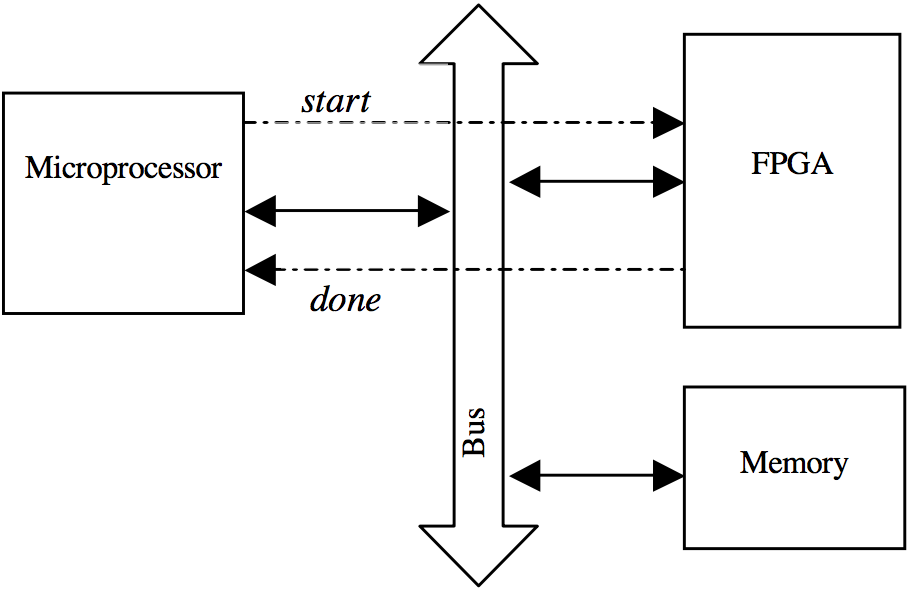
\includegraphics[width=0.35\textwidth]{img/into-soc.png}
		\caption{Visão geral de um CSoC.}
		\label{fig:i-soc}
	\end{figure}

	O conceito de CSoC é importante quando necessita da construção de sistemas computacionais que podem utilizar de circuitos com processadores como é o caso de sistemas embutidos.

	% embedded
    \todo[inline]{A parte de wearable vc tem q explorar mais no capitulo 1 tb, como construcao da motivacao. Uma introducao tem q ser a sequinte sequencia}
	Os sistemas computacionais embutidos são produtos que utilizam processadores e podem estar desde fornos de microondas, até sistemas de controle de aeronaves.
	Requerem técnicas na qual difere das utilizadas para \design\ de computadores de propósito geral ou aplicações de \software\ dessas máquinas \cite{Wolf1994}.
	Em 2015, foi previsto um total de 6,5 bilhões de dispositivos ativamente conectados para o ano de 2016 segundo notícias da empresa de pesquisa e consultoria Gartner \cite{RobvanderMeulen2015}.

	% wearable
	No âmbito de sistemas embutidos, existe um subconjunto na qual possui o propósito de integrar ao sistema corporal expandindo suas capacidades.
	Esses sistemas, chamados de sistemas \wearables, envolvem grande volume de dados de múltiplos sensores complexos ou outros sistemas e são requeridos para prover serviço autônomo contínuo em um longo período de tempo.
	Tais dispositivos demandam de uma alta performance e/ou baixo consumo de energia, sem apresentar \textit{trade-off} de confiabilidade e segurança. %\cite{Jozwiak2017}
	%
	Segundo \cite{Jozwiak2017}, com computação de alta performance e estudos em gasto energético eficiente, foi possível a facilitação do rápido progresso da computação móvel e autônoma.
	Tudo isso deve-se à possibilidade de comunicar-se com a rede global de comunicação, combinada com o progresso de sensores e atuadores, criando novas oportunidades importantes de projeto.
	Exemplos disso são indústrias inteligentes, cidades e casas, bem como setores de \textit{internet} das coisas (IoT, do inglês \textit{Internet of Things}), sistemas móveis como automóveis inteligentes, computação móvel como \textit{smartphones}, comunicação e, não menos importante, os sistemas computacionais \wearable.
	Sendo uma tecnologia pertencente ao conjunto de sistemas embutidos, o sistema computacional \wearable\ pode ser definido como `embutidos que foram inseridos em ambiente \mobile\ de seus usuários, não exercendo a mesma atividade'.
	Um desafio de \design\ para sistemas \wearable\ é combinar a flexibilidade de demanda pelos vários ambientes e aplicações fins de uso e a alta performance exigida em tarefas com o baixo consumo de energia requerido para maximizar o tempo de uso da bateria.


\todo[inline]{1- Apresnetar o problema:}
	% intro particionamento
	A redução do ciclo de comercialização de um produto e o aumento de sua eficiência de desenvolvimento de projeto tem se tornado uma preocupação na área de \design\ de sistemas embarcados, o que inclui os \wearables.
	A técnica de particionamento \hs\ tem sido uma das principais tecnologias para o desenvolvimento de sistemas embarcados desde que, este afeta a performance do sistema como um todo. Para \cite{Hassine2017}, uma das soluções mais elegantes na computação que provê otimizações sistêmicas sobre essas circunstâncias é por meio do particionamento \hs.
	Segundo \cite{Wolf1994}, sistemas embutidos é considerado único pelo fato da necessidade de um \codesign\ de \hs, visando performance, custo e metas de confiabilidade.

	Um exemplo simbólico pode ser ilustrado na Figura \ref{fig:rt-edwards_partitioning} no qual um módulo em \software\ é substituído por um componente em \hardware\ executando a mesma tarefa mas com maior performance.

	\begin{figure}[!b] \centering
		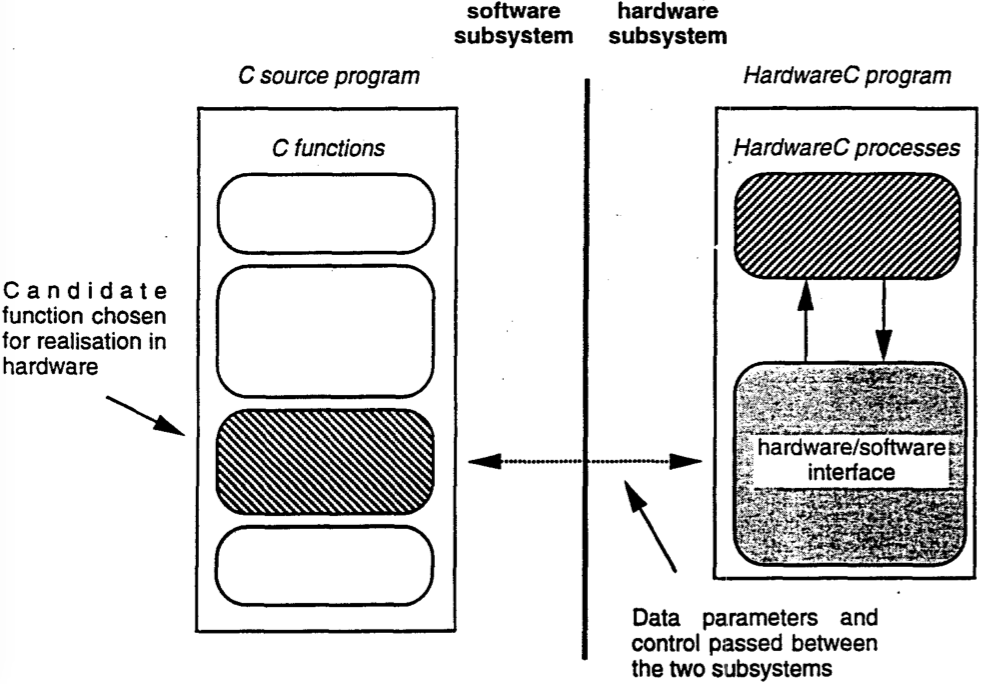
\includegraphics[width=0.37\textwidth]{img/rt-edwards_partitioning.png}
		\caption{Ilustração de um particionamento. Fonte: \cite{Edwards1994}.}
		\label{fig:rt-edwards_partitioning}
	\end{figure}

	\cite{Hidalgo1997} dizem que o objetivo principal do particionamento \hs\ é o balanceamento de todas as tarefas de forma a otimizar alguns objetivos de sistema sobre determinadas restrições.
	A ideia do particionamento é agrupar específicos conjuntos de instruções em uma aplicação e então mapear esses grupos tanto em \hs.
	Os grupos designados ao \software\ são executados sequencialmente pelo respectivo processador do sistema enquanto os mapeados em \hardware\ são implementados por uma combinação customizada ou por circuitos sequenciais \cite{Sass2010}.

	% particionamento
	Quando necessita de performance ao realizar o \codesign\ (termo referente ao inglês \textit{Participatory Design}) de \hs\ para sistemas embutidos, o problema de qual função do sistema deverá ser implementada em \hardware\ ou em \software\ emerge e esse problema é conhecido por particionamento \hs\ (\textit{hardware/software partitioning}).
	Um significante esforço foi posto nesta área nos últimos dez anos, segundo \cite{Trindade2016}.


\todo[inline]{2- Justificativa pq eh um problema relevante:}

	Tradicionalmente, o particionamento é feito manualmente, mas com o desenvolvimento de \designs\ mais complexos em sistemas embarcados, esse problema de decisão torna-se cada vez mais um desafio para os \designers\ de projeto \cite{Trindade2016}.
	Segundo \cite{Edwards1994}, as pesquisas em \codesign\ de \hs\ têm como objetivo o \design\ de sistemas heterogêneos.
	Assim, a meta principal é reduzir o tempo de até a disposição do produto ao mercado bem como a redução do custo dos produtos projetados no qual um projeto de produto normalmente inclui a especificação sistêmica, estimação de custo, o particionamento \hs, a síntese de ambos os projetos e sua simulação \cite{Wolf1994}.

\todo[inline]{3- Motivacao pra resolver este problema:}

	Descrevendo um pouco mais sobre, com o desenvolvimento de complexos \design\ em sistemas embutidos, o particionamento \hs\ tornou-se um problema de otimização em \codesign\ de sistemas \cite{Yan2017}. Tal problema que envolve \design\ colaborativo e multidisciplinar, é um passo chave no \design\ de modernos produtos embutidos \cite{Trappey2016}. Implementações que baseiam-se somente em módulos de \software\ possuem mais flexibilidade e são menos custosas, entretanto, seu custo eleva-se em termos de tempo de execução, o que já não acontece no mundo de \design\ de projetos em \hardware\ \cite{Zhang2008, Hassine2017, Wolf1994}.

	Como o grande requisito para eficiência necessariamente segue junto com a alta velocidade de processamento, existem vários métodos que abordam o problema de particionamento \cite{Arato2005} desde métodos manuais quanto a utilização de meta-heurísticas.

	Dessa forma, ao utilizar o FPGA para o problema de particionamento, é possível acelerar uma aplicação em \hardware\ na qual pode fornecer uma ordem de magnitude de melhoria no desempenho e eficiência de energia em comparação com o \software\ que está sendo executado inteiramente em um processador \cite{Cong2009, Lo2009, Zhang2008a}. Um exemplo de sucesso é o anúncio da Microsoft em \cite{Putnam2014} na qual aceleraram o \textit{Bing Search} em duas vezes com a utilização de FPGAs em seus \textit{data centers} \cite{Putnam2014} além da aquisição da Altera, uma das duas maiores vendedoras de FPGAS no mundo, pela Intel em \cite{Maan2015} por cerca de $ 16.7 $ bilhões de dólares \cite{Maan2015}.


\todo[inline]{4- Contribuicao ao resolver o problema:}


\todo[inline]{5- Objetivos:}

\subsection{Objetivos da Dissertação}
	Este trabalho tem como objetivo a apresentação do problema de particionamento \hs\ bem como sua importância no mundo de sistemas computacionais embutidos, com foco em sistemas \wearables\ apresentando algumas soluções utilizadas atualmente \todo{e a solução proposta}.

    \begin{itemize}
    	\item Introduzir o projeto de sistemas computacionais \wearable;
        \item Apresentação da abordagem metodológica para o uso da solução do problema ao aplicado no contexto desses sistemas.
    \end{itemize}


\subsection{Organização da Dissertação}
	Os demais capítulos deste trabalho estão organizados da seguinte forma: No Capítulo \ref{chap:revisao_bibliografica} é apresentada uma revisão bibliográfica do problema, abordando alguns métodos de fundamental importância para este trabalho. No Capítulo \ref{chap:relacionados} são descritos alguns trabalhos relacionados ao tema abordado. No Capítulo \ref{chap:desenvolvimento} são apresentadas as metodologias. No Capítulo \ref{chap:experimentos} \todo{são?} apresentados os resultados e suas considerações para o problema. No Capítulo \ref{chap:conclusao} são apresentadas as conclusões finais e propostas de trabalhos futuros.

\section{Revisão Bibliográfica} \label{chap:revisao_bibliografica}

\subsection{FPGAs e Sintetizadores em Alto Nível}

%Neste capítulo será descrito os principais conceitos necessários para o entendimento base dos fundamentos do trabalho, além de suas tecnologias e metodologias.

%\subsection{\textit{Field-Programmable Logic Device} (FPGA)}

	% uso de fpga no mundo
	Até recentemente, os \hardwares\ reconfiguráveis eram utilizados unicamente na prototipação de projetos de circuitos integrados de aplicação especifica (ASIC) e produção em baixo volume por causa de sua baixa velocidade e custo por unidade.
	Mas com a variedade desses dispositivos disponibilizados hoje no mercado, em conjunto com a elevação do custo de engenharia não recorrente, houve um crescente interesse na utilização de FPGAs para sistemas embutidos devido suas vantagens sobre ASICs em termos de flexibilidade de projeto e custo zero de engenharia não recorrente \cite{Mei2000}. 
	%lousa branca
    \begin{comment}
	Tais dispositivos, juntos com sua plataforma de interação, de forma geral, permitem ao \designer\ de sistemas embutidos ter uma \textit{lousa branca} em que possa implementar \hardwares\ computacionais personalizados tão facilmente como o desenvolvimento de um \software, como foi possível ilustrar na Figura \ref{fig:rt-board}.
	% Plataforma FPGA
	Dessa forma, uma \textit{plataforma FPGA} é um chip na qual contém o componente FPGA integrado à inúmeras interfaces e componentes desde LEDs (do inglês \textit{Light-Emitting Diode}) e \textit{switchs} até porta Ethernet e interface vídeo VGA (do inglês \textit{Video Graphics Array}) e como possui recursos suficientes para circuitos complexos, é possível implementar funções de processamento de imagem, interfaces de rede, algoritmos criptográficos e processadores completo de acordo com sua capacidade. %\cite{Plessl2003}
	Entretanto, enquanto configurar um \hardware\ reconfigurável é uma tarefa fácil graças às ferramentas disponíveis hoje, criar um \design\ de \hardware\ inicial não é \cite{Sass2010}.

	\begin{figure}[h] \centering
		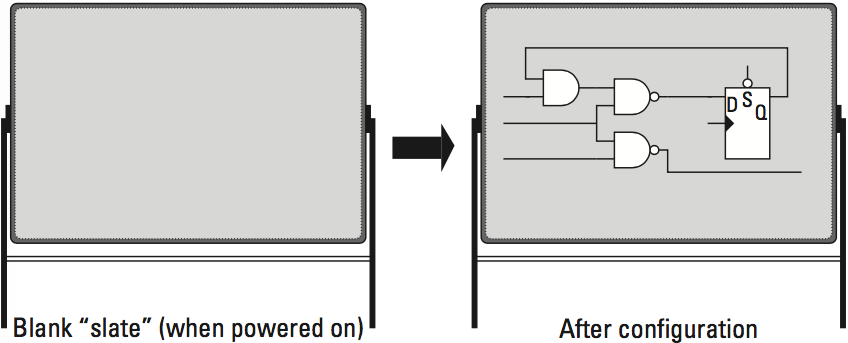
\includegraphics[width=0.75\textwidth]{img/rt-board.png}
		\caption{Ilustração em alto nível do funcionamento interno do FPGA. Fonte: \cite{Sass2010}.}
		\label{fig:rt-board}
	\end{figure}

	A seguir, será descrito a tecnologia que consiste os \hardwares\ reconfiguráveis, em especial o FPGA, e as respectivas linguagens de descrição de \hardware.

	\subsubsection{\textit{Field-Programmable Logic Device} (FPGA)}
		% PLD
		Para introduzir alguns conceitos, é importante destacar o que são os dispositivos lógicos programáveis (PLDs, do inglês \textit{Programable Logic Devices}). Às vezes chamados de dispositivos lógico programáveis em campo (FPLD, do inglês \textit{Field-Programmable Logic Device}), podem ser adaptados para criar muitos dispositivos digitais, desde simples portas lógicas até estruturas complexas. \cite{tocci2003sistemas, Plessl2003} dizem que com um investimento de capital pequeno, qualquer empresa pode comprar os \software\ de desenvolvimento e \hardware\ necessário para programar PLDs para seus projetos digitais. De modo geral, os PLDs são descritos como pertencendo a três tipo diferentes sendo eles os dispositivos lógicos programáveis simples (SPLD), dispositivos lógicos programáveis complexos (CPLDs, do inglês \textit{Complex Programmable Logic Devices}) e arranjo de portas programáveis em campo (FPGA) sendo o último tipo abordado neste trabalho \cite{Brown1996}.

		%LUTS
		Os FPGAs em especial constituem de vários módulos lógicos programáveis relativamente pequenos e independentes interconectados para criar funções maiores. Cada módulo lida, normalmente, com até quatro ou cinco variáveis de entrada. A maioria dos FPGAs utilizam uma \textit{look-up table} (LUT) para criar as funções lógicas desejadas. Uma LUT funciona como uma tabela-verdade, no sentido que a saída é programada para criar a função combinacional armazenando valores verdadeiros e falsos adequado a cada combinação de entrada.
		Os recursos de roteamento de sinal programável dentro do chip tendem a ser bem variados, com extensões de caminhos diferentes disponíveis. Os atrasos de sinal em um projeto dependem do roteamento real de sinal selecionado pelo \software\ de programação. Os módulos lógicos também contêm registradores programáveis. Eles não são associados a nenhum pino de entrada e saída (I/O, do inglês \textit{Input and Output}). Em vez disso, cada pino de I/O é conectado ao bloco programável de entrada e saída que, por sua vez, é conectado aos módulos lógicos com linhas de roteamento selecionadas.
		\todo{figura fpga}
        Os blocos de I/O podem ser configurados para fornecer recursos de entrada, saída ou bidirecionais, e registradores internos, usados para guardar dados que entram ou saem. Uma arquitetura geral de FPGA com 16 blocos lógicos é exibida na Figura \ref{fig:rt-arch_fpga}.
        Todos os blocos lógicos e os de entrada e saída implementam qualquer circuito lógico. As interconexões programáveis são estabelecidas por meio de linhas que passam pelas linhas e colunas nos canais entre esses blocos \cite{tocci2003sistemas}.
	%A tecnologia interna de um FPGA consiste basicamente de um arranjo de blocos lógicos, canais de roteamento para interconexão de blocos lógicos e blocos de entrada e saída de sinais em torno do circuito.
	FPGAs baseado em SRAM (do inglês \textit{Static Random Access Memory}) utilizam células SRAM para controlar a funcionalidade de blocos lógicos e entrada e saída de sinais bem como as rotas, e pode ser reprogramado arbitrariamente em nível de circuito, muitas vezes, baixando um novo \textit{stream} de dados de configuração para o dispositivo.
	Hoje, esses dispositivos possuem milhões de portas de lógica programável, bilhões de transistores, além de outros blocos de \hardware\ dedicados dedicados como rápidas memórias embarcadas e multiplicadores de ponto-fixo tornado-o um dos circuitos integrados (CI) mais densos existente \cite{Choi2016}.
    \end{comment}

		\begin{comment}

		\begin{figure}[h] \centering
			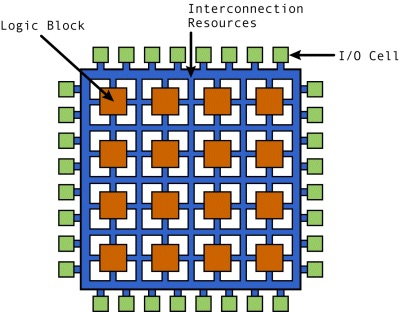
\includegraphics[width=0.5\textwidth]{img/rt-arch_fpga.jpg}
			\caption{Exemplo da arquitetura internas de um FPGA. Fonte: \url{http://www.eetimes.com/document.asp?doc_id=1274496}. Acesso: 30/05/2017.}
			\label{fig:rt-arch_fpga}
		\end{figure}
		\end{comment}


	\begin{comment}
		% tecnologia e energia
		Segundo \cite{tocci2003sistemas}, tais maravilhas de flexibilidade de projetos digital utilizam tecnologia CMOS e podem fornecer uma série de opções de projeto sendo voltados para indústria e até mesmo educação. 
        Ao utilizar tecnologia CMOS, o consumo de energia do chip é relativamente baixo comparado com outras tecnologias podendo ser confeccionado em nível de tensão elétrica, frequências e cargas para os sinais de I/O. O mercado fornece diferentes graus de velocidade de FPGA a fim de que o projetista utilize o mais adequado ao projeto.

		Um dispositivo FPGA pode ser configurado para um número infinito de projetos, de maneira que não é possível simplesmente afirmar o montante de dissipação de energia para um dispositivo FPGA. %O \software\ Quartus II tem duas ferramentas para estimular o montante de uso de energia para uma aplicação. %O \textit{PowerPlay Early Power Estimator} é usado durante os estágios iniciais do projeto para estimar a magnitude de potência do dispositivo.
		Dessa forma, FPGAs são chips que podem ser programados instantaneamente para funções de qualquer circuito digital \cite{Choi2016}.
    \end{comment}

		% Importancia
		Os autores \cite{tocci2003sistemas, Plessl2003} citam que o motivo de PLDs estarem dominando o mercado é o fato de que, como são dispositivos programáveis, a mesma funcionalidade pode ser obtida com um circuito integrado (CI), em vez de com diversos circuitos individuais. 
        Isso significa menor espaço ocupado na placa, menor consumo de energia, maior confiabilidade, menor complexidade de desenvolvimento e, geralmente, menor custo de fabricação.

		%Um das maiores barreiras para o \design\ de projetos em FPGA é a necessidade de uso de linguagem de Descrição de \Hardware\ (do inglês \textit{Hardware Description Language}). HDL é uma das classes de linguagens de computação usados para descrever formalmente um circuito eletrônico. Uma expressão padrão baseada em texto HDL é capaz de descrever o comportamento temporal ou a estrutura de circuito (espacial) de um sistema eletrônico. Sua origem veio da raiz da necessidade de documentar o comportamento do \hardware \cite{Sass2010}.

		%HDL é amplamente utilizado em \design\ de \hardware\ especificando detalhes de \design\ de chip para tantos chips específicos quantos os próprios FPGAs. Para customizar algum tipo de algum chip lógico digital específico, HDLs especifica um modelo para um comportamento específico de um circuito antes do circuito ser projetado e construído. Ferramentas lógicas de sínteses são invocadas em seguida para gerar informações geométricas que são utilizadas para produzir as máscaras \textit{photolithographic}, necessárias para a fabricação do CI do projeto desenvolvido.

		%A utilização de uma HDL é o primeiro passo no processo de síntese. O código é entregue ao compilador lógico, chamado de ferramenta de síntese, e sua saída será carregada ao dispositivo reconfigurável.
		%A propriedade única deste processo e que fornece a lógica programável em geral é que, com esse processo, é possível alterar o código HDL muitas vezes, compilá-lo e fazer seu \textit{upload} no mesmo dispositivo para testar quantas vezes forem necessárias sem custo adicional \cite{Smith1998}.

		Enquanto a maioria de engenheiros de \hardware\ utilizam tanto o \textit{VHDL} quanto o \textit{Verilog}, na qual possuem um nível elevado de complexidade \cite{Choi2016}, existe outras linguagens disponíveis para uso como \textit{SystemC}, \textit{HandelC} e \textit{Impulse}. Fornecem a construção de sistemas \hs\ juntos, dando ao \designer\ uma linguagem de alto nível para manuseio do projeto \cite{Sass2010}.


	%\subsection{\textit{High-Level Synthesis} (HLS)}
		Sintetizadores em Alto Nível (HLS, do inglês \textit{High-Level Synthesis}) são procedimentos que sintetizam códigos em alto nível para HDLs. Realizado uma especificação de \design\ em \software, um HLS pode reduzir os longos ciclos do processo de \design\ de \hardware\ e ainda trazer melhoria em performance e eficiência energética \cite{Choi2016}.

		As primeiras ferramentas sistetizadores baseavam em linguagem \textit{C} mas não houve um sucesso em seu uso pois os engenheiros de \hardware\ acreditam que existe uma lacuna entre o HLS e o \design\ de \hardware\ feito por humanos por parte das ferramentas HLS não explorarem profundamente o recurso de paralelismo, além de que, para os engenheiros de \software\ HLS continua sendo uma dificuldade já que muitas partes do projeto, como a integração do sistema, permanecem em grande parte como um processo manual. Ferramentas como o \textit{framework} LegUp possuem o propósito de entregar um bom HLS além de tentar amenizar esses problemas de projetos \cite{Canis2013}.

		Para prover um melhor suporte para o paralelismo em \hardware, utilizaram de bibliotecas \textit{multi-threads} como a \textit{Pthread} \cite{Barney2009}, \textit{OpenMP} \cite{openmp}, OpenCL \cite{Trevett2008} para criar aceleradores em \hardwares\ paralelos. É investigado otimizações em memória e arquitetura de sistema provendo melhorias em performance de circuito, área, utilizando uma abordagem do padrão produtor-consumidor para inferir circuito de transmissão em \hardware.

\begin{comment} %comment Módulos e Interfaces em \Design\ de \Software
\subsection{Conceitos e Componentes de \Design\ de Sistemas}
	% \subsubsection{Módulos e Interfaces}
	%Existem duas filosofias de \design\ para a construção de um sistema. Em um delas é possível realizar a especificação de cada função do projeto, chamado de blocos básicos\footnote{Um bloco básico é uma sequência maximal de instruções sequenciais com \textit{single entry and single exit} (SESE).}, e conectá-los logicamente de acordo a fim gerar o sistema completo. Tal é descrito como abordagem \textit{bottom-up}.
	%A segunda baseia-se na descrição de um sistema completo e geral sendo que, em seguida, o \designer\ desmembra-o definindo seus sub-blocos até chegar ao nível mais básico de suas funções. Essa é chamada de abordagem \textit{top-down}.
	%O conceito de abordagem de desenvolvimento de projetos é importante para descrever os conceitos de módulo e interface.%, segundo \cite{Sass2010}.



	\subsubsection{Módulos e Interfaces em \Design\ de \Software}
		\cite{Sass2010}, em seu livro, descreve que módulo é qualquer conjunto de operação auto-contidas que possui um nome, interface formal e geral e alguma descrição funcional. Isso significa que qualquer procedimento, mesmo que em \software\ ou em descrição de \hardware, que possa ser representado por uma caixa graficamente é considerado um módulo.
		Define-se por interface formal o nome do módulo e a enumeração de duas operações, incluindo suas entradas e saídas, caso existam e a interface geral inclui todas as características da interface formal e qualquer protocolo ou comunicação adicional implícita. Com a interface formal descrita, é possível realizar inspeções mecânica e técnica no módulo enquanto a geral, o entendimento desse em alto nível.
		Por último, um módulo pode ter também uma descrição funcional no qual pode ser implícita, formal ou informal. Quando a descrição é implícita, a descrição está presente de forma clara no nome do módulo, como por exemplo \texttt{full\_adder}. A formal consiste na documentação ou em meios matemáticos e comentários formais sobre as operações do módulo e a informal pode ser comentários descritivos ao longo da escrita da função.

		Outros termos importantes são implementação e instância. Uma implementação é a realização de uma funcionalidade pretendida de um módulo mesmo que este tenha várias implementações como é permitido num ambiente de descrição de \hardware\ criar várias arquiteturas diferentes para um mesmo módulo.
		Já a instância é o uso de uma implementação.
		Enquanto em instâncias em nível de \software\ imagina-se relações um-a-um entre implementação e instância, em \hardware\ é comum o uso de copias físicas de cada implementação, sendo cada cópia representa uma instância no final. Na Figura \ref{fig:instance} é possível ver em \textit{a)} um instância padrão de uma implementação e em \textit{b)} uma outra instância com uma identificação única.

		\begin{figure}[h] \centering
			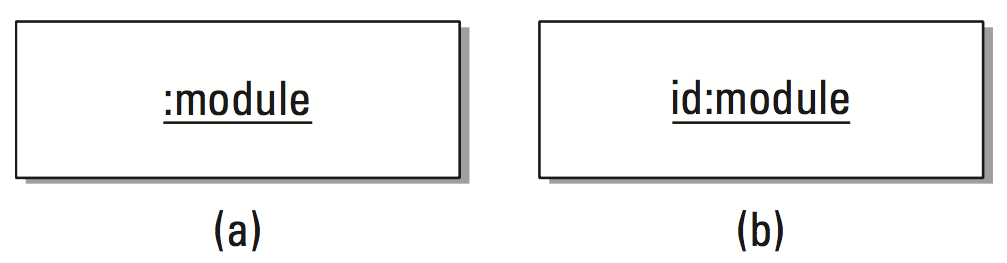
\includegraphics[width=0.7\textwidth]{img/f3-2.png}
			\caption{Instâncias e suas descrições. Fonte: \cite{Sass2010}.}
			\label{fig:instance}
		\end{figure}

		Como exemplificação, pode-se construir um somador completo de 4-bit utilizando várias instâncias da implementação do somador completo de 1-bit, exibido na Figura \ref{fig:somador_instancias}.

		\begin{figure}[h] \centering
			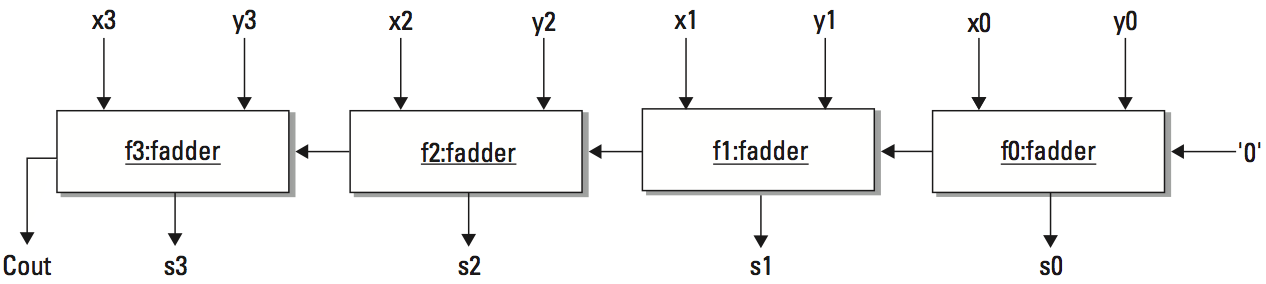
\includegraphics[width=0.98\textwidth]{img/f3-3.png}
			\caption{Somador completo 4-bit utilizando instâncias de 1-bit. Fonte: \cite{Sass2010}.}
			\label{fig:somador_instancias}
		\end{figure}
	\end{comment}

\begin{comment}
	\subsubsection{Abstração e Estado}
	\subsubsection{Coesão e Acoplamento}
\end{comment}


\subsection{Ferramenta \Profile} \label{sec:profile}

		\Profile\ é uma técnica para coletar informações do \software\ em tempo de execução. O \software\ referencial é executado com uma entrada representativa e o tempo gasto em várias partes da aplicação é mensurado. 
        %A Figura \ref{fig:f4-1} exibe um exemplo gráfico de \profile\ de \software\ em um codificador de imagem.

		Uma das técnicas do \profile\ de mensurar uma aplicação é realizar interrupções periódica no programa e amostrar o seu \textit{program counter}. Dessa forma, é possível utilizar um histograma para contar quando um programa é interrompido em um endereço particular e a partir dessa informação, calcular a fração aproximada do tempo total de execução gasto em suas partes. Distribuições GNU/Linux possuem a ferramenta \texttt{gprof} que realiza o cálculo de tais informações de \software\ \cite{Graham1982}.



\subsection{Sistemas Computacionais \Wearables}
	% Introdução histórica e geral
	Sistemas computacionais \wearables\ são sistemas que, com a possibilidade de ter um computador acoplado ao corpo, proporciona-se ao usuário um nível superior de informações contextualizadas dentro de um ambiente interativo \cite{Amorim2017}.

	\todo{intowearaable}

	Devido ao movimento de seus usuários, um computador \wearable\ é embutido em um ambiente \mobile\ e necessita-se da interação com seu ambiente ao seu redor \cite{Plessl2003}.
	Um sistema \wearable\ é composto por um conjunto de nós distribuídos e uma rede de comunicação centralizada num módulo principal, sendo possível determinar, por exemplo, a geração de eletricidade por meio de geradores \textit{piezo-electric} integrados aos sapatos, energizando uma parte do sistema \wearable\ com o caminhar do usuário \cite{Kymissis1998} ou a ação do usuário por meio de acelerômetros \cite{VanLaerhoven2002, Kern2002}.

	Com a distribuição espacial dos módulos pelo corpo, a comunicação torna-se um item importante em termos consumo de energia \cite{Kymissis1998}. A rede de comunicação é uma mistura de conexões cabeadas e sem-fios. Para dispositivos \wearables, a comunicação sem-fio é a tecnologia predominante \cite{Plessl2003}.

	A introdução desses sistemas no ambiente de pesquisa não é nova como é reportado por \cite{Sutherland1968}, \cite{Mann1996} e \cite{Mann1997}. Entretanto, a aplicação desses, depende diretamente da miniaturização dos componentes eletrônicos. Esse fenômeno é claro com o crescente espaço ganho nas indústrias e nas atividades pessoais de usuários pelos \textit{smartwatches}, \textit{fitness trackers}, óculos, equipamentos de realidade virtual e aumentada e muitos outros. Com esses novos dispositivos de propósito geral minituarizados, aumenta-se a sua atração devido à fácil disponibilidade dos dispositivos, baixo preço e ferramentas de desenvolvimento disponíveis para desenvolvimento de aplicações específicas incluindo compiladores e sistemas operacionais para tal, mas não são otimizados para uso \wearable.
	\cite{Plessl2003} cita que em \cite{Plessl2003}, muitos dos sistemas \wearables\ construídos possuíam características diferentes de componentes que prestam auxílio em tarefas pessoais de usuários, citados anteriormente.
	Por exemplo, o uso dados de teclados, canetas para entrada de dados ou um \textit{display} LCD contradiz com o paradigma de operações \textit{hands-free} e a propriedade de computação \wearable\ discreta.
	Sistemas de computação distribuídos no corpo construídos a partir desses equipamentos são altamente ineficientes devido à falta de especialização de componentes individuais de propósito específico.
	Dessa forma, a computação \wearable, seguindo esse conceitos, se define muito bem como um subconjunto de sistemas embutidos.

	% Característica de um dispositivo wearable
	\subsubsection{Característica de um \Wearable}

		A caracterização de um dispositivo \wearable\ é feita acordando às classificações pré-estabelecidas em relação à suas funcionalidades e requisitos de \hardware. O mercado possui um número considerável de dispositivos \wearables\ que são utilizados em inúmeras áreas e mesmo que cada equipamento separado tenha suas próprias características, muitas soluções em \hardware\ compartilham uma arquitetura e organização de recursos implementados interna comum.
		Esses detalhes também podem ser expandidos às características relativas a recursos de sistemas operacionais, no qual dispositivos \wearables\ podem ser classificados além de seus componentes de \hardware\ internos como suas funções de performance \cite{Delabrida2016, Amorim2017}, como representado pela Figura \ref{fig:classification}.

		\begin{figure}[h] \centering
			\vspace{-10pt}
			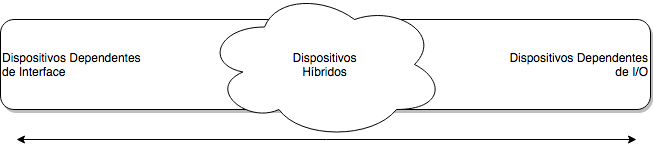
\includegraphics[width=0.45\textwidth]{img/rt-gradiente.png}
			\vspace{-10pt}
			\caption{Classificação de sistemas \wearables. De um extremo existe os dispositivos dependentes de interfaces de usuário e do outro os dependentes de entrada e saída de sinais enquanto entre eles, a gama de combinações possíveis.}
			\label{fig:classification}
		\end{figure}

		De um lado desta gama de dispositivos existem os dispositivos dependentes de interfaces de usuário que possuem alta dependência com operações interfaces gráficas, provendo respostas sobre as interações do usuário.
        Esses dispositivos focam principalmente em tarefas para renderização em \textit{displays} como por exemplo equipamentos de realidade virtual e aumentada para implementação de objetos tridimensionais.

		De outro lado existem os dispositivos dependentes de entrada e saída de sinais. Esses dispositivos atuam principalmente com o estímulo por algum dado oriundo de outro dispositivo ou do ambiente assim entregue à nuvem respeitando restrições de tempo real.
        Isso se da pela utilização de sensores acoplados ao dispositivo que podem exigir uma boa vazão de dados e pequena latência como são os monitores de atividade remota, situação na qual cria-se o ambiente perfeito para o termo conhecido por \textit{Internet of Things} (IoT).

		Entre dispositivos dependentes de interfaces de usuário e de entrada e saída de sinais existe os híbridos. São dispositivos que utilizam recursos de ambos os extremos citados.
        Dispositivos como \textit{Smartwatches} e \textit{fitness trackers} são exemplos de tais dispositivos híbridos no qual possuem restrições de equalização a prioridade dada pelo dispositivo para ambas as operações de interface e sinais.

		A separação dos conceitos computação \wearable\ e IoT ainda não estão claros segundo a bibliografia. Sistemas operacionais de propósito específico para ambientes \wearable\ são comumente focado em um único tipo de seguimento de produto como os \textit{smartwatches} sendo um meio que proporciona aos desenvolvedores um meio para sua aplicação final além de entregar um produto de alta qualidade.
        Entretanto, atualmente não existe nenhum sistema que satisfaça todos os requisitos apresentados \cite{Amorim2017}.

		Já \cite{Jozwiak2017} em seu trabalho caracteriza um sistema \wearable\ como um sistema \textit{cyber}-físico\footnote{Sendo \textit{cyber-} uma combinação dos termos `computador', `rede de computadores' ou  `realidade virtual' com um segundo termo, no caso o `físico' oriundo de circuitos.} móvel autônomo.
        São sistemas que podem ter mobilidade inerente ou poder ser transportado para outro sistema, industrial ou natural (incluindo humanos), sendo autônomos em termos de funcionalidade.
        Podem ser utilizados para aplicações de consumidores (computação móvel), extensões ou reposição de capacidades humanas, sistemas sociais (\textit{health-care} inteligente), automotivo, industrial (monitoramento) e aplicações comerciais como realidade aumentada para informações turísticas.
		Eles representam uma grande parte da heterogeneidade de sistemas embarcados, cobrindo muitos campos e tipos de aplicações que vão desde um dispositivo inteligente integrado à roupa, focado no campo de computação \textit{mobile} pessoal, até indústrias como dispositivos de segurança. % \cite{Jozwiak2017}.
        Esses dispositivos podem também trabalhar de forma colaborativa com \textit{smartphones}, redes e outros sistemas criando um sistema mais complexo.

		Segundo \cite{VanLaerhoven2002}, a distribuição de sensores se adequ à pesquisa que aumenta objetos mundanos com elementos computacionais, comumente designados por computação ubíqua, o que afirma também que computação \wearable\ também não foge do conceito uma vez que superfícies de roupas são uma plataforma de suporte ideal para uma grande quantidade de sensores (desde que sejam miniaturizados para que eles não obstruam o usuário).
		Essa restrição de tamanho geralmente significa que a própria qualidade do equipamento também está comprometida, o que leva ao conceito de muitos atuadores e sensores simples.

		Sistemas \wearables\ são uma subclasse de sistemas embutidos distribuídos e por causa disso, são sujeitos à várias restrições de \design sendo elas performance em multi-nós, gasto energético consciente e alta flexibilidade \cite{Plessl2003}:
        \begin{itemize}
        	\item \textbf{Performance de multi-nós:} Requerem um performance base fixa para tarefas que não mostram altas demandas computacionais nem restrições de tempo rigorosa.
            Sistemas \wearables\ executam rajadas de tarefas de computação intensiva que consideram restrições de tempo-real. Não realizando as tarefas, o sistema torna-se inaplicável.

			\item \textbf{Gasto energético consciente:} É essencial em sistemas na medida que ele deve-se manter ativo e funcional num certo período de tempo. O \design\ do gasto de energia conduz inúmeros desafios como gerenciamento computacional energético eficiente e energização dinâmica. Diferenciando os termos de baixo custo de energia e eficiência energético, o consumo de energia é mensurado pela divisão da dissipação energética pelo tempo mensurado.

            A eficiência energética relaciona o total de energia necessário para computar uma tarefa específica sendo o desafio a construção de um \design\ na qual possui-se alta eficiência energética para um dado conjunto de tarefas. O procedimento dinâmico de energização consiste na tarefa de associar determinada tarefa para o componente mais eficiente (energeticamente falando) disponível e forçar todos os outros não utilizados pelo sistema a serem postos em modo de economia de energia ou desligá-los quando apropriadamente.

			\item \textbf{Flexibilidade:} Quando menciona-se sobre alta flexibilidade, é considerado o fato de que o dispositivo será utilizado em situações altamente dinâmicas. Isso fica claro na necessidade na qual os requisitos de aplicação variam de acordo com as escolhas do usuário, mas também com o contexto e local utilizado. Outro é no fato de que o usuário troca de roupas constantemente e com isso os dispositivos devem ter a capacidade de serem acoplados e removidos, neste caso. Isso além de critérios como confiabilidade, disponibilidade e fatores dependentes de sua forma como volume e peso.
        \end{itemize}

		Dessa forma, pode-se estabelecer que os requisitos flexíveis em um sistema \wearable\ demanda um sistema de computação programável de propósito geral, enquanto os requisitos de alta performance e consumo de energia consciente demandam um sistema computacional especializado. Dessa forma, como meio para solução desses problemas, \cite{Plessl2003} utilizaram-se de um \hardware\ reconfigurável para incoporar ao sistema. O trabalho exibe um sistema \wearables\ compreendendo de um processador de até médio porte em termos de processamento e módulos reconfiguráveis.
		A utilização de \hardware\ reconfigurável nos permite alcançar alto processamento com maior eficiência energética em relação à processadores para tarefas de computação intensiva em tempo real.

\section{Trabalhos Relacionados} \label{chap:relacionados}

	%O particionamento \hs\ encontra-se em duas principais bordagens sendo essas algoritmos para otimização de escolhas de particionamento e uso de recursos de determinada aplicação e o particionamento para sistemas embutidos.

	%not embedded
	O particionamento de forma geral é um problema de otimização na qual vários autores utilizam métodos para auxiliar na decisão de cada componente do \design\ referencial de \software. Utiliza-se tanto algoritmos exatos quanto heurísticas \cite{Arato2005}.

	\begin{figure}[!b] \centering
    	\vspace{-15pt}
		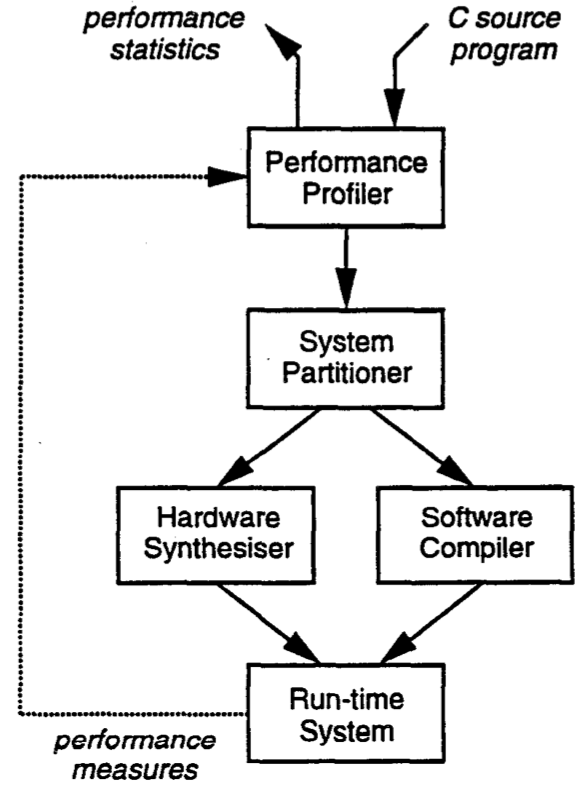
\includegraphics[width=0.21\textwidth]{img/rt-edwards_method.png}
        \vspace{-10pt}
		\caption{Metodologia de \codesign\ de \cite{Edwards1994}. Fonte: \cite{Edwards1994}.}
		\label{fig:tr-edwards_method}
	\end{figure}
	Os autores \cite{Edwards1994} utilizam do particionamento para aprimorar a performance do seu \software. Em seu trabalho, realiza-se a tentativa de tratar regiões críticas da aplicação na qual uma solução em \software\ não pode chegar à restrições de performance requeridas e uma solução em \hardware\ deve ser encontrada, ou a performance total pode ser acelerada pela implementação de uma região crítica em \hardware.
	Em seu trabalho, é apresentada uma metodologia para desenvolvimento \codesign\ no qual consiste na construção do código de uma aplicação em \textit{C} e as regiões críticas são identificadas e particionadas. Feito isso realizar-se mensurações do projeto e uma nova verificação de particionamento é realizada, como é exibido na Figura \ref{fig:tr-edwards_method}.
	Utiliza-se também de um FPGA para as mensuras de performance e a propriedade de reconfiguração para novos testes em \hardware.

	Já o trabalho de \cite{Stitt2003} procura uma abordagem utilizando métodos de otimização de \software\ dinâmicos, introduzindo a primeira abordagem para particionamento de \hs\ dinâmico.
	O processo consiste na deteção da região de \software\ mais frequentemente executada e reimplementa-a em \hardware\ de FPGA.
	Eles afirmam que a utilização de particionamento dinâmico trás uma série de vantagens comparado com abordagens tradicionais.

    Existem vários trabalhos que propuseram algoritmos exatos baseados em \textit{branch-and-Bound} \cite{Jigang2004, Mann2007, Strachacki2008}, programação dinâmica \cite{Madsen1997, Wu2006} e linear inteira (ILP, do inglês \textit{integer linear programming}) \cite{Niemann1997}.

	\cite{Nematbakhsh_theeffect} parte para o exame da relação entre o \textit{footprint} gerado para o FPGA e o \speedup\ do \software\ na situação na qual um FPGA é utilizado para a implementação de \textit{loops} e sub-rotinas críticas.
	Como utilizam uma abordagem direta, utilizaram de ferramentas protótipos e comerciais como \textit{Synopys' Nimble Compiler} e \textit{Proceler}, para a facilitação do processo.

	Abordagens mais recentes como a de \cite{Yan2017} usa o método de particionamento \hs baseado em otimização \textit{position disturbed particle swarm} com otimização invasiva de \textit{weed}.

	\cite{Wang2016} citam que o particionamento depende da exploração de caracterização, estimação e \design\ espacial das métricas de custo e performance sistêmica. É exaltado também que o \codesign\ nos dias de hoje é tão complexo que a simplificação do particionamento só para duas partes não é suficiente para a representação do problema como um todo. Sobre essa crítica, dissertam sobre a inclusão de parâmetros chave de \design\ e uso de recursos que deveriam ser incorporados à modelagem do sistema e dessa forma, o trabalho proposto por eles visa considerar a modelagem de incerteza para particionamento de sistemas com um conjunto melhorado de parâmetros para compartilhamento de recursos \hs.
	Esse terceiro item a ser considerado ao problema de particionamento podem ser definidos em três tipos sendo essas: \textit{a)} o conjunto de recursos necessários para particionar uma dada tarefa (sendo esses RAM, ROM, DPS, blocos IP do inglês, \textit{intelectual propriety}, entre outros); \textit{b)} tarefaz que possuem vários parâmetros de configurações que provê diferentes \textit{trade-off} entre recursos e performances como por exemplo circuitos de multiplicações/divisões que podem ser sintetizados sequencialmente (pouca área e lento) ou combinatório\footnote{Por \textit{unrolling}, técnica de otimização de código no qual tenta reduzir ou eliminar as iterações de determinado \textit{loop} do código.} (muita área e rápido); \textit{c)} a dificuldade da mensura de desempenho e impacto no uso de recursos em várias configurações de partição com precisão precisando ter em mente a partição com a natureza incerta dessas estimativas não precisas.
	A teoria da incerteza é uma abordagem que é um sistema matemático que é designado para modelar indeterminância ao invés do uso da teoria da probabilidade. Isso pois, quanto tem-se muitas amostras de uma quantidade indeterminada, seria significativo a utilização da teoria de probabilidade ou \textit{fuzzy} pela propriedade de serem contínuas entre o intervalo 0 (zero) à 1 (um). Entretanto, se não possui-se amostras suficientes para a estimação de uma distribuição de probabilidade, utiliza-se do conhecimento do domínio para avaliação do grau de crença de que cada evento indeterminado acontecerá, no caso, aplicado pela teoria da incerteza. A teoria da incerteza é um ramo da matemática axiomática para modelagem de graus de crença, de modo geral.

	Como outro trabalho recente que aborda o particionamento, \cite{Choi2016} descreve um \textit{framework} chamado LegUp.
	Com essa ferramenta é possível compilar um \software\ e suas \textit{threads} gerando um sistema \textit{hardware-only} ou também um sistema híbrido particionado paralelo utilizando aceleradores, gerando também todos os itens necessários para tal como memórias sintetizadas e sistemas de interconexões. Utilizam duas técnicas de descrição de paralelismo em \software\ sendo elas a \textit{Pthreads} e a \textit{OpenMP} sendo a primeira permite a sintetização de funções operando concorrentemente em \hardware\ com aceleradores, e a segunda usada para gerar os próprios aceleradores executados concorrentemente em um sistema de compartilhamento de memória.
	Afirmam também que a sua ferramenta produz HDL de alta performance que pode ser comparado com circuitos que são gerados por ferramentas HLS comerciais.

	Entretanto, além de todo arcabouço de algoritmos para escolhas para sistemas de propósito geral tal como os citados, existe uma subconjunto específico do problema na qual trata-se do particionamento em sistemas embutidos.


	% Embedded
	O desenvolvimento para sistemas \hs\ participativo para sistemas embutidos ou microcontroladores já é pesquisado amplamente como os trabalhos de \cite{Ernst1993, Gupta1995, Hardt1995, Gajski1994, Bolsens1997}, publicados na década de 90.
	\cite{Mei2000} em seu trabalho, descreve um particionamento de \hs\ além de uma abordagem de escalonamento para sistemas embutidos dinamicamente reconfiguráveis (DRESs, do inglês \textit{dynamically reconfigurable embedded systems}) no qual possuem como projeto um processador de propósito geral junto com um FPGA sendo este reconfigurável em tempo de execução para reduzir custos. Dessa forma, seu trabalho consiste numa análise de tempo de configuração e, como contribuição, a análise do tempo de reconfiguração parcial do FPGA.
	%Com a adição da reconfiguração parcial de \hardware, o escalonamento no FPGA torna-se um problema de alocação restrita, enquanto o escalonamento em circuitos integrados de aplicação específica (ASICs, do inglês \textit{application-specific integrated circuits}) é um problema de serialização.
	Para o escalonamento, \cite{Mei2000} utiliza um método baseado na heurística do algoritmo genético (GA, do inglês \textit{genetic algorithm}) e num algoritmo de escalonamento de lista com melhorias.
	O escalonador desenvolvido atua como uma sub-rotina do algoritmo de particionamento. Ele é invocado no passo \textit{evolution} do GA. Além do escalonamento já conhecido em processador e barramento sequenciais determinando a ordem e tempo início de execução, o algoritmo também deve fazer o escalonamento no FPGA. Mas não só determinando o tempo de início da tarefa, mas sim sua posição no FPGA respeitando as restrições de recursos e precedentes, tornando assim o problema uma abordagem ao problema de alocação restrita.

	Já \cite{Arato2003} descreve algumas versões diferentes do problema de particionamento, correspondendo à sistemas de tempo-real e custo restringido, respectivamente fornecendo análise matemática formal para o problema, provando que são problemas $ \mathcal{NP} $-difícil no caso geral. Apresentaram uma abordagem baseada na programação linear inteira resolvendo o problema de forma otimizada, mesmo para sistemas de grande porte, além de outra abordagem utilizando a heurística GA na qual encontrar soluções próximas ao ótimo para sistemas largos.

	\cite{Mann2007}, em \cite{Mann2007}, descreveram uma primeira tentativa para um algoritmo exato, não heurístico, para o problema de particionamento. Eles utilizam um esquema na qual utilizam a estratégia \textit{branch-and-bound} como um \textit{framework}, permitindo o incremento de outros algoritmos. Em sua implementação, realizaram várias investigações para incrementar a eficiência do algoritmo, incluindo várias técnicas sendo elas: \textit{lower bounds based on LP-relaxation}, uma mecânica de inferência customizada, condições não-triviais necessárias baseadas num algoritmo \textit{minimum-cut}, e diferentes heurísticas com passos pré-otimizados. O algoritmo também pode ser generalizado a fim de incluir mais de uma restrição, podendo também o \designer\ prescreva quais nós devem estar em qual nível de projeto. Eles demonstram que o produto pode resolver problemas de particionamento altamente complexos em tempo razoável. Citam que é cerca de dez minutos mais rápido que algoritmos exatos anteriores baseados em programação linear inteira para os testes realizados.

	Pesquisas mais recentes como a de \cite{Hassine2017}, em \cite{Hassine2017}, procuravam aplicar otimizações sobre o tempo de execução e gasto energético para \cores\ baseados em sistemas embarcados por meio de algoritmos de particionamento.
	O algoritmo proposto é destina-se a alcançar um particionamento de grafos à procurar o melhor conjunto da relação energia e tempo de execução.
	Testado em comparação com outros algoritmos heurísticos como \textit{Simulated Annealing}, Busca Tabu e Genético, o algoritmo mostra-se ser melhor adequado para aplicações em \cores\ baseados em sistemas embarcados que necessitam do equilíbrio no \textit{tradeoff} de sistemas embarcados.

	\cite{Trindade2016} por exemplo utiliza do GA para solucionar o problema de particionamento em sistemas embutidos. Em seu trabalho, é proposto novas abordagens para o problema usando técnicas de verificação baseadas nas teorias de módulo de satisfação (SMT, do inglês \textit{satisfiability modulo theories}). Apresentam um exemplo de particionamento, modelam e solucionam-o usando três diferentes técnicas sendo a principal ideia é aplicar mo método de verificação SMT ao particionamento \hs, e por fim, comparar os resultados com técnicas de otimizações tradicionais como ILP e GA.

	\cite{Jozwiak2017} em seu \textit{survey} publicado em \cite{Jozwiak2017}, considera vários aspectos de uma aplicação embutida, bem como suas tecnologias de \design\ com foco sistemas móveis modernos e \wearables.
	É citado dois paradigmas de desenvolvimento para sistemas embutidos sobre sistema de multi-processadores heterogêneos sendo eles o paradigma de sistemas \textit{life-inspired} e sistemas \textit{quality-driven}. O paradigma de sisetmas \textit{life-inspired} especifica princípios básicos, características e organização funcional e estrutural de um sistema embutido por meio da analogia à vida de um organismo inteligente, além de básicas soluções de mecanismos e arquiteturas de sistemas para implementar tais princípios. Já o paradigma de sistemas \textit{quality-driven} (ou seja, orientado pela qualidade) torna-se uma segunda solução para o \design\ de dispositivos que necessitam satisfazer as exisgências de \textit{real-time}, baixo consumo de energia, entre outros. Dessa forma, especifica-se qual a nova qualidade do sistema a ser requeria e como esta meta é obtida. De forma a facilitar a compreensão, \cite{Jozwiak2017} define qualidade de uma solução sistemica proposto como o total de sua eficácia e eficiência na resolução do problema real. Eficácia entende-se como o grau em que uma solução atinge seus objetivos e a eficiência o grau em que uma solução usa recursos para realizar seus objetivos e juntas determinam o grau de excelência. Elas são expressas em termos de parâmetros mensuráveis, o que é necessário para implementar o design \textit{quality-driven}. Entretanto, é descrito ao final que, enquanto \designers\ aprenderam bastante na construção de plataformas de \hardware\ heterogêneos altamente paralelos, os métodos e ferramentas automatizadas para a sua programação e o paralelismo do algoritmo, bem como o \codesign\ coerente da arquitetura \hs\ ainda são atrasados perante à tecnologia.
	Por fim, o \textit{survey} não menciona nenhuma pesquisa feita sobre particionamento para sistemas \wearables.

\begin{comment}
	\subsection{Análise de Performance de Sistema}
\end{comment}


\section{Metodologia da Pesquisa}

\subsection{\Design\ Referencial de \Software\ para Sistemas Embutidos Utilizando Grafo de Controle de Fluxo} \label{chap:design} \label{sec:GCF}

	Segundo \cite{Sass2010} é possível descrever um sistema quanto em \hardware\ ou em \software\ livre de uma especificação de forma. 
    Uma delas é o desenvolvimento de rápidos protótipos referenciado como \design\ de referência de \software.
	Sua vantagem mais notável é a generalização de uma especificação de projeto bastante completa, eliminando qualquer tipo de incertezas sobre o comportamento do sistema com o simples fato de analisar o \design\ referencial do \software.
	% além de outras como o fato de que sua especificação pode ser analisada por ferramentas computacionais, e gerando modelos aut.

	%Assumindo que o \design\ de referência de \textit{software} já exista,
	%Aqui será demonstrado matematicamente como computação está em \design\ referencial de \software\ para que depois, isso possa nos auxiliar na decisão do que deverá ser implementado em nível de \hs. 
    Como o sistema a ser particionado é dado em forma de grafo de tarefas/rotinas, utiliza-se da teoria de grafos \cite{Mann2007}, em especial o gráfico de controle de fluxo (GCF). 
    Ele é definido por $ G = (B, F) $ onde $ B $ são vértices que representam os blocos básicos e $ F $ são arestas que indicam a todas as possibilidades de caminhos entre os blocos. 
    %Um exemplo é exibido na Figura \ref{fig:blocos_basicos}. O primeiro grupo \A\ é um bloco não básico porque não é maximal, ou seja, a primeira instrução \texttt{store word with update} deveria estar incluída ao grupo. Grupo \B\ é um bloco básico e o grupo \C\ não é pois existe duas entradas para o bloco, sendo elas na instrução \texttt{store word} e também pelo \texttt{branching} direcionado para \texttt{L2}.

	%Fazendo uma relação entre código em alto nível até o grafo de controle de fluxo, a Figura \ref{fig:f3-6} \textit{a)} exibe os blocos básicos em um código sem funcionalidade útil. Na Figura \ref{fig:f3-6} \textit{b)} é exibido o código gerado por um compilador para \texttt{PowerPC}\footnote{Arquitetura que utiliza RISC como arquitetura do conjunto de instruções.} onde os blocos básicos são identificados e por fim o gráfico de controle de fluxo, representado pela Figura \ref{fig:f3-6} \textit{c)}. Deve-se atentar que, só é possível identificar blocos básicos em um arquivo em linguagem de programação \textit{C} desde que se saiba qual compilador foi utilizado para emitir o código \assembly.
	\begin{comment}
	\begin{figure}[h] \centering
		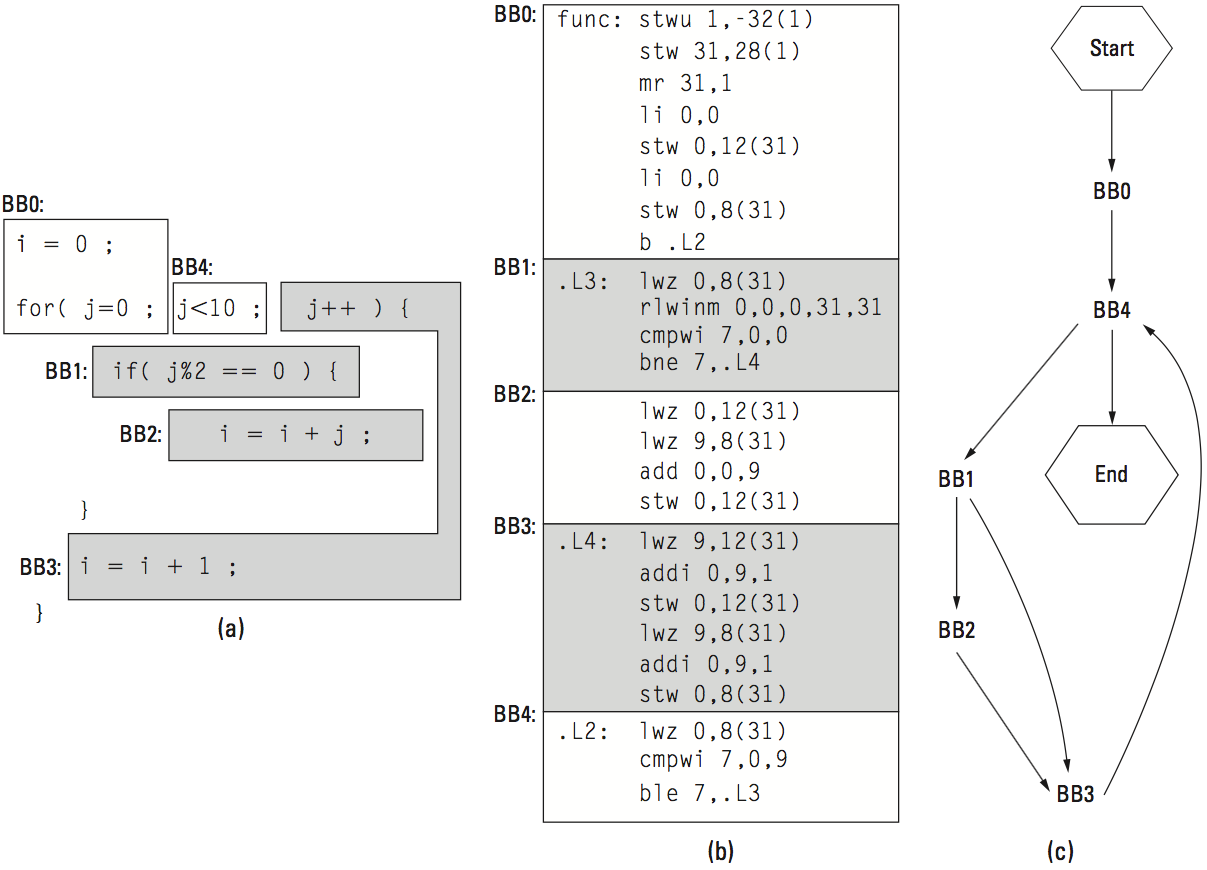
\includegraphics[width=0.9\textwidth]{img/f3-6.png}
		\caption{Identificação de blocos básicos e a representação de cada modelo de descrição de \software.}
		\label{fig:f3-6}
	\end{figure}
    \end{comment}

	Com a decomposição de um \design\ de referência de \software, gera-se dois componentes: uma porção a ser realizada em \hardware\ e outra executada em \software\ e essa decisão de divisão é chamada de problema de particionamento (descrito na Seção \ref{chap:desenvolvimento}).
    %Para sistemas baseados em Plataformas FPGA, particionamento é um sub-problema de um problema mais geral localizado no \codesign, onde refere-se ao \design\ cooperativo envolvendo \textit{stakeholders}, por exemplo.

	%Para continuar, deve-se definir alguns conceitos básicos, descritos na Seção \ref{sec:gc}.

\subsection{Grafo de Chamada} \label{sec:gc}
		\cite{Arato2003, Arato2005} \cite{Mann2007} \cite{Hassine2017} \todo{a} 
        
        Explicado como é modelado sub-rotina de um \design\ referencial de \software\ utilizando o grafo de controle de fluxo, agora será descrito o grafo de chamada (GC). Consiste num conjunto de GCFs, um por sub-rotinas, ou seja,

		\begin{equation}
			\mathcal{C} = {C_0, C_1, \dots C_{n-1}}
		\end{equation}

		%onde $ C_i = (V_i, E_i) $
		onde $ C_i = (B_i, F_i) $ representa o grafo de controle de fluxo de uma sub-rotina $ i $. Sendo assim, o grafo estático de chamada da aplicação é escrito por

		\begin{equation}
			\mathcal{A} = (\mathcal{C}, \mathcal{L}) \label{eq:a}
		\end{equation}

		onde $ \mathcal{A}$ representa uma aplicação específica e $ \mathcal{L} \subseteq \mathcal{C} \times \mathcal{C} $ é um subconjunto do plano cartesiano dos GCF. Duas sub-rotinas são relacionadas se podem ser determinadas, no tempo de compilação, que a sub-rotina $ i $ tem potencial de invocar a sub-rotina $ j $, ou seja, $ (C_i, C_j) \in \mathcal{L} $.

		É assumido que os blocos básicos de cada sub-rotina são disjuntos, ou seja, cada bloco básico em uma aplicação pertence a exatamente um GCF. Além do mais, é assumido que um nó raiz para o GC é implícito, ou seja, uma sub-rotina é designada a iniciar a execução.

		%Nem todos os executáveis podem ser expressados nesse modelo. Por exemplo, o manuseio de sinais e interrupções não são representadas e assim, não é possível determinar todos vértices $ F_i $ em uma dada sub-rotina $ C_i $ de um GCF antes da execução. 
        %Uma outra forma é com o paradigma de orientação à objeto. Ele depende do tempo de execução para conectar os métodos virtuais invocados e dessa forma, por \design, esse paradigma nos previne de saber todos os vértices antes da execução.
        %Para agora, será considerado que o modelo é suficiente para ser expressado em \design\ referencial de \software.

		Um equívoco comum é de que uma definição formal de particionamento só aplica à separação de aplicação componentes de \hs, ou seja, a partição contém exatamente dois conjuntos. 
        Todavia, para fazer o problema mais tratável, é comum agrupar primeiramente operandos em recursos, ou seja, uma partição com um grande número de subconjuntos, e então mapeia esses recursos tanto em \hardware\ quanto \software. 
        Assumindo que esses recursos atuam razoavelmente bem \textit{clustered}, então a decomposição de uma aplicação em componentes de \hs\ pode ser dirigida por comparações de ganho de performance desse recurso contra outro situado no outro conjunto. \todo{reler}

		Uma partição $ \mathcal{S} = \{S_0, S_1, \dots\}$ de um conjunto universal $ U $ é um conjunto de subconjuntos de $ U $ sendo que

		\begin{equation}
			\bigcup_{S \in \mathcal{S}} S = U \label{eq:part_form_1}
		\end{equation}
		\begin{equation}
			\forall S, S' \in \mathcal{S} | S \cap S' = \emptyset \label{eq:part_form_2}
		\end{equation}
        e assim
		\begin{equation}
			\forall S \in \mathcal{S} \cdot S \neq \emptyset \label{eq:part_form_3}
		\end{equation}

		A Equação \ref{eq:part_form_1} mostra que cada elemento de $ U $ é um membro de, pelo menos, um subconjunto $ S \in \mathcal{S} $. As Equação \ref{eq:part_form_2} e \ref{eq:part_form_3} dizem que os subconjuntos $ S \in \mathcal{S} $ são emparelhados disjuntos e não vazio. Em outras palavras, cada elemento do nosso universo $ U $ termina exatamente em um dos subconjuntos de $\mathcal{S}$ e nenhum dos subconjuntos são vazios.
		\begin{comment}
		Por exemplo, considerando as vogais da língua inglesa onde o universo $ U = \{a, e, i, o, u, y\} $. Assim, uma partição desse problema $ \mathcal{X}_a $ de $ U $ pode ser representado por


		\begin{equation}
			\mathcal{X}_a = \left\{\{a, e, i, o, u\}, \{y\}\right\} \label{eq:xa}
		\end{equation}

		e supondo que o conjunto pode ser representando por cada unidade, uma outra forma de representação pode ser


		\begin{eqnarray}
			\mathcal{X}_b &=& \left\{\{a\}, \{e\}, \{i\}, \{o\}, \{u\}, \{y\}\right\}
		\end{eqnarray}

		Sobre tais conceitos, a Partição \ref{eq:part_c} viola a Equação \ref{eq:part_form_1} e a Partição \ref{eq:part_d} viola as Equações \ref{eq:part_form_2} e \ref{eq:part_form_3}.

		\begin{eqnarray}
			\mathcal{X}_c &=& \left\{\{a\}, \{e\}, \{i\}, \{o\} \right\} \label{eq:part_c} \\
			\mathcal{X}_d &=& \left\{\{a, e, i\}, \{i, o, u, y\}, \{\}\right\} \label{eq:part_d}
		\end{eqnarray}

		A Figura \ref{fig:f4-2} ilustra o $ \mathcal{X}_a $ graficamente, segundo a Partição \ref{eq:xa}.

		\begin{figure}[h] \centering
			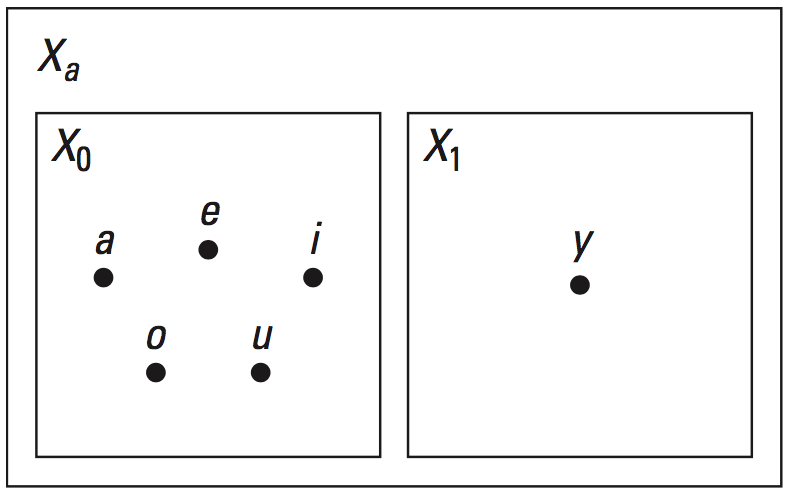
\includegraphics[width=0.5\textwidth]{img/f4-2.png}
			\caption{Figura representativa do mapeamento da aplicação.}
			\label{fig:f4-2}
		\end{figure}
		\end{comment}
		Aprendido os conceitos, é possível aplicar o formalismo à $ \mathcal{A} $. Se assumirmos que nosso universo é o conjunto de todos os blocos básicos $B$ de todas as sub-rotinas, então $U$ é as partições de sub-rotinas

		\begin{equation}
			U = \bigcup_{C \in \mathcal{C}} B(C) \label{eq:bigcup}
		\end{equation}

		 e chamaremos de partição natural da aplicação, onde
{ \footnotesize
		\begin{equation}
			\mathcal{S}  = \left \{
			\underbrace{\left \{ b_0, b_1, \dots, b_i \right \}}_{\text{sub-rotina }C_0},
			\underbrace{\left \{ b_i, b_{i+1}, \dots \right \}}_{\text{sub-rotina }C_1},\dots
			\underbrace{\left \{ b_j, b_{j+1}, \dots \right \}}_{\text{sub-rotina }C_{n-1}}
			\right \}
		\end{equation}
}

		Nossa tarefa será reorganizar a partição de blocos básicos e então mapear cada subconjunto de ambos os \hardwares\ e \software. Dessa forma, estamos livres para criar e remover subconjuntos não vazios, e mover blocos básicos ao redor até termos uma nova partição e assim termos um novo resultado $ \mathcal{A}’ = (\mathcal{C}’, \mathcal{L}’) $, inferido a partir da reorganização da partição $ \mathcal{X}’ $. O segundo passo é mapear cada subconjunto de $ \mathcal{X} $ para ambos \hs\ como é exibido abaixo

{ \tiny 
		\begin{equation}
			\mathcal{X}' = \left \{
			\underbrace{
            		\underbrace{
                    	\left \{ b_j, b_{j+1}, \cdots \right \}
                       }_{\text{sub-rotina }C_k}
                    \underbrace{
                    	\left \{ b_k, b_{k+1}, \cdots \right \}
                    }_{\text{sub-rotina }C_l}
                    \dots
                }_{\text{\software}}
                \
			\underbrace{
            		\underbrace{
            			\left \{ b_0, b_1, \cdots, b_i \right \}
                    }_{\text{sub-rotina }C_r}
                    \underbrace{
                        \left \{ b_i, b_{i+1}, \cdots \right \}
                    }_{\text{sub-rotina }C_s}
                    \dots
                }_{\text{\hardware}}
			\right \} \label{eq:part_final}
		\end{equation}
}


\subsection{Ganho de Performance} \label{sec:ganho_performance}
	Para explicar como performance pode ser utilizada para guiar o particionamento, será descrita uma métrica simples chamada taxa de execução.
	É parcialmente motivada pelo fato de que: \textit{a)} o ganho de performance é relativamente fácil de ser mensurado e \textit{b)} por causa de que, de todas as métricas comumente utilizadas, \speedup\ é frequentemente a mais importante. Diferente do mundo \software\ onde se tem análise de ordem de complexidade, em \hardware\ não possui-se um guia geral para comparação. O ganho de performance para aplicações em geral pode estar na acumulação de pequenos ganhos que deveriam ser perdido numa aplicação direta na teoria de complexidade.

	% tempo software
	Assim, será usado a informação de \profile\ (Seção \ref{sec:profile}) para coletar o tempo total de execução, bem com uma fração do tempo gasto em cada sub-rotina.
    O produto disso é a aproximação entre o tempo necessário para executar uma porção de aplicação em \software\ e usar isso como o tempo que se espera que tomará em futuras execuções. 
    Será utilizado $ s(i) $ para representar o tempo de execução esperado para uma invocação de uma sub-rotina $ i $, ou seja, bloco básico. 
    É considerado uma aproximação pois é dependente dos conjuntos de dados de entrada para muitas aplicações além da existência de erros que podem impactar a performance.

	% tempo hardware
	Precisa-se também aproximar o tempo que uma implementação equivalente em \hardware\ que iria tomar. 
    No caso dos blocos básicos implementados, isso é frequentemente mais preciso. 
    Como não possui-se um controle de fluxo, uma ferramenta auxiliar à síntese pode dar uma aproximação de acurácia de propagação de tempo.
    %Ou, se o recurso é \textit{pipelined}, o número de estágios é mais precisamente conhecido. Caso o recurso inclua controle de fluxo mas não contenha nenhum \textit{loop}, pode-se considerar o caminho mais longo como uma estimativa conservativa.

    Recursos com um número variável de iterações através de um \textit{loop} apresentam o maior obstáculo para encontrar um tempo de \hardware\ aproximado. 
    Nesse caso, implementação e \textit{profiling} com recurso em \hardware\ pode ser a única solução. 
    Independente, assume-se que uma aproximação apropriada $ h(i) $ para o existente tempo de execução em \hardware.

	% tempo mudanca de estado, configuracao, latencia
	Por fim, a interfaceação entre \hs\ requer tempo e este custo também precisa ser contabilizado. Pode-se aproximar deste custo pela aproximação do montante total do estado que necessita ser transferido ou o custo de configuração e latência. Em ambos os caso, são representados por $ m(i) $ para recursos $ i \in \mathcal{H} $, sendo $\mathcal{H}$ o conjunto de recursos do \hardware.

	% y é speedup
	%Taxa de execução é a velocidade na qual um sistema computacional completa uma aplicação, e em um sistema de plataforma FPGA olhamos para o \hardware\ para melhorar sua taxa de execução.
    O ganho, ao comparar uma solução \hs\ contra uma solução puramente \software, é tipicamente mensurado como \speedup. Utilizamos $ \gamma $ para sua representação e isso nos permitirá comparar recursos diferentes contra outros para determinar melhores particionamentos.
    Dessa forma, qualquer subconjunto de blocos básicos que não produzem um ganho de performance, podem ser excluídos de consideração. Em outras palavras, somente subconjuntos de blocos básicos para qual $ \gamma > 1.0 $ são considerados recursos candidatos.

	%Em geral, não mensuramos taxa de execução\footnote{Taxa de execução é a velocidade na qual um sistema computacional completa uma aplicação.}, mas ao invés disso, o tempo de execução, que no caso é inverso.
	Então quando considerado se um conjunto particular de blocos básicos deveriam ser mapeados ao \hardware\ ou \software, estamos interessados em seu ganho em \speedup. Mais especificamente, interessa-se no ganho de performance individual de cada recurso e assim, definindo $ \gamma(i), i \in \mathcal{C} $

	\begin{equation}
    	\gamma(i) = \frac{s(i)}{h(i) + m(i)}
    \end{equation}

	onde $ h(i) $ e $ s(i) $ são o tempo de execução de uma implementação de um recurso $ i $ em \hs\ e a função $ m(i) $ é o tempo que se leva para sincronização, ou seja, o tempo que leva para guiar um dado entre o processador e o item reconfigurável.

	%Assumindo por um momento que usaremos esse recurso separado em nosso \design, deve-se questionar sobre o quão rápido é a aplicação.
    A velocidade da aplicação é dependente dos ganhos de performance do recurso e o quão frequentemente ele é utilizado no \design\ referencial de \software. Pode-se ter essa fração do tempo gerado de um recurso particular $ p(i) $ a partir de informações de \textit{profile} e dessa forma o \speedup\ da aplicação no geral será

	\begin{equation}
    	\Gamma = \left [
        	(1 - p(i))
            	+
            \frac{
            	p(i)
            }{
            	\gamma(i)
            } \right ]^{-1}
    \end{equation}

	A inversão representa que estamos movendo entre tempo de execução e taxa de execução para manter o sentido de ganho de performance.

	A partir dessa equação, podemos observar que aumentando a velocidade do \hardware\ de um único recurso tem-se menos e menos impacto na performance da aplicação a medida que sua frequência decresce.
    
	\subsubsection{A Considerações de Recursos} \label{sec:recursos}

    Para aumentar a performance sistêmica de uma aplicação no geral, também deve-se aumentar o sistema com múltiplos recursos que aumentará a performance de componentes individualmente assim como aumentando a fração agregada de tempo gasto em \hardware.
    Para computar o \speedup\ de múltiplos recursos em \hardware, deve-se avaliar o ganho sistêmico de um conjunto de recursos $ \mathbb{D} $ onde cada membro do conjunto contribui à performance do sistema baseado na fração do tempo gasto em cada característica.
    Para estimar a performance desta partição, podemos adicionar recursos e rearranjar os termos para ter um ganho de performance almejado no geral, assim para o cálculo de performance dos recursos, utiliza-se da Equação \ref{eq:d_final}.

	\begin{equation}
    	\Gamma (\mathbb{D}) =
        \left [
        	1 + \sum _{i \in \mathbb{D}} \left (
            	\frac{
                	p(i)
                }{
                	\gamma(i)
                } \ – \ p(i)
                \right)
        \right ]^{-1} \label{eq:d_final}
    \end{equation}

		Seguindo a Equação \ref{eq:d_final}, uma tentativa seria adicionar recursos na abordagem $\sum_i p_i$, ou seja,  implementar tudo em \hardware\ para maximizar a performance, ignorando todos os custos de desenvolvimento e recursos limitados.
		Num FPGA, há um número finito de recursos disponíveis para implementação de circuitos em \hardware. Tais recursos são limitados e a maioria das aplicações realísticas irão exceder esse limite disponível.
		Um meio de aproximação de recursos é contar o número de células lógicas requeridas para cada recurso. Um chip que terá um valor escalar $ r_{FPGA} $, representará o total de números de células lógicas disponíveis. Então $ r(i) $ pode ser usado para representar a quantidade de células lógicas requeridas por cada recurso $ i $. Fazendo uma simples relação, tem-se que $ \sum_{i \in \mathbb{D}} r(i) < r_{FPGA} $ 
		\begin{comment}
			\begin{equation}
				\sum_{i \in \mathbb{D}} r(i) < r_{FPGA}
			\end{equation}
		\end{comment}
		restringe quão largo $ \mathbb{D} $ pode crescer.

		Sabendo que dispositivos modernos são heterogêneos, uma típica plataforma FPGA tem múltiplos tipos de recursos além de células lógicas como memória, blocos DSP, etc. podendo ser representado por um vetor de recursos

		\begin{equation}
			\vec{r}_{FPGA} =
				\begin{pmatrix}
				r_{Logic\ Cells} \\
				r_{Memory}\\
				r_{DSP}\\
				\vdots \\
				r_{n-1}
				\end{pmatrix}
		\end{equation}

		e com isso, $\sum_{i \in \mathbb{D}} \vec{r}(i) < \vec{r}_{FPGA}$
        \begin{comment}
		\begin{equation}
			\sum_{i \in \mathbb{D}} \vec{r}(i) < \vec{r}_{FPGA}
		\end{equation}
        \end{comment}
		onde $ \mathbb{D} $ é o conjunto de recurso incluídos no \design.

		%Infelizmente\todo{a}, esse modelo não leva em consideração o fato de que alguns recursos alocados podem interferir em outros, além de que a estimativa de performance é frequentemente baseada na suposição que recursos são próximos um do outro e recursos de rotas não são parte integral do modelo.







\begin{comment}

\section{Transferência de Estado} \label{chap:tranferencia}

\subsection{Transferência de Estado}
	Segundo \cite{Sass2010}, manter estado consistente sobre dispositivos FPGA e processadores é um desafio.
    Isso pois, como cada FPGA tem sua própria hierarquia de memória independente, estados são amplamente distribuídos no \design\ e há ampla variedade de interconexões entre FPGA e processadores.
    Assim, isso significa menos estados para serem transferidos e grande variedade de mecanismos disponíveis.
    Os tipos de estados serão descritos a seguir pois são requisitos para identificação de qual parte do estado da aplicação precisa ser explicitada pela comunicação processador e recurso.
    %Para entender melhor deve-se definir dois conceitos sendo eles estado afetado e preso ajudando a decidir quais partes do estado da aplicação necessitam de ser explicitamente comunicados entre processador e recurso.

	\begin{description}
		\item [Estado Afetado:]
		Na computação alguns estados são independentes pela construção e não precisam de ser transferidos de lugares. Retirando tais estados, restam os estados afetados.

        Esses, são os dados da aplicação que, durante a transferência de controle, podem ser modificados ou lidos por um recurso ou processador, necessitando de ser consistente entre todas as distribuições.
		%Estados afetados podem existir em grande escala. Principalmente quando arranjos, estruturas de dados complexas ou ponteiro estão envolvida e podem ser acessados de várias formas possíveis e geralmente não é possível saber se dois ponteiros estão apontando para um mesmo endereço.

        \item [Estado Preso:]
        Acontece quando parte da hierarquia de memória é compartilhada, nem todo o dado tem que ser explicitamente transferido e assim, caso todo o estado corrente esteja em memória primária (RAM) e ambos os dispositivos possuem acesso a ela, então não existe razão para a transferência explícita dos dados.

        Processadores modernos são construídos com quantidade significativa de memória que podem ser utilizadas como parte de estado sem a atualização da memória primária.
        Compiladores naturalmente utilizam toda a vantagem de registradores para armazenar os estados.

        Implementações em \hardware\ também incorporam dados ao longo do projeto e seus registradores e \textit{flip-flops} possuem valores intermediários entre ciclos de \textit{clock} dentro do projeto.
        O estado de uma aplicação é armazenado em várias partes do sistema.
        Para um recurso implementar parte de uma aplicação, precisa-se então integrar-se com parte do estado.

        Esse pode ser considerado mais facilitado pelo fato de que o estado está localizado em um espaço comum. Mas se um estado está localizado num registrador ou em uma cache de um processador, ele não pode ser acessado pelo sistema externo e, neste caso, o estado encontra-se preso e deve ser explicitamente transmitido pela interface.

		\begin{figure}[h] \centering
			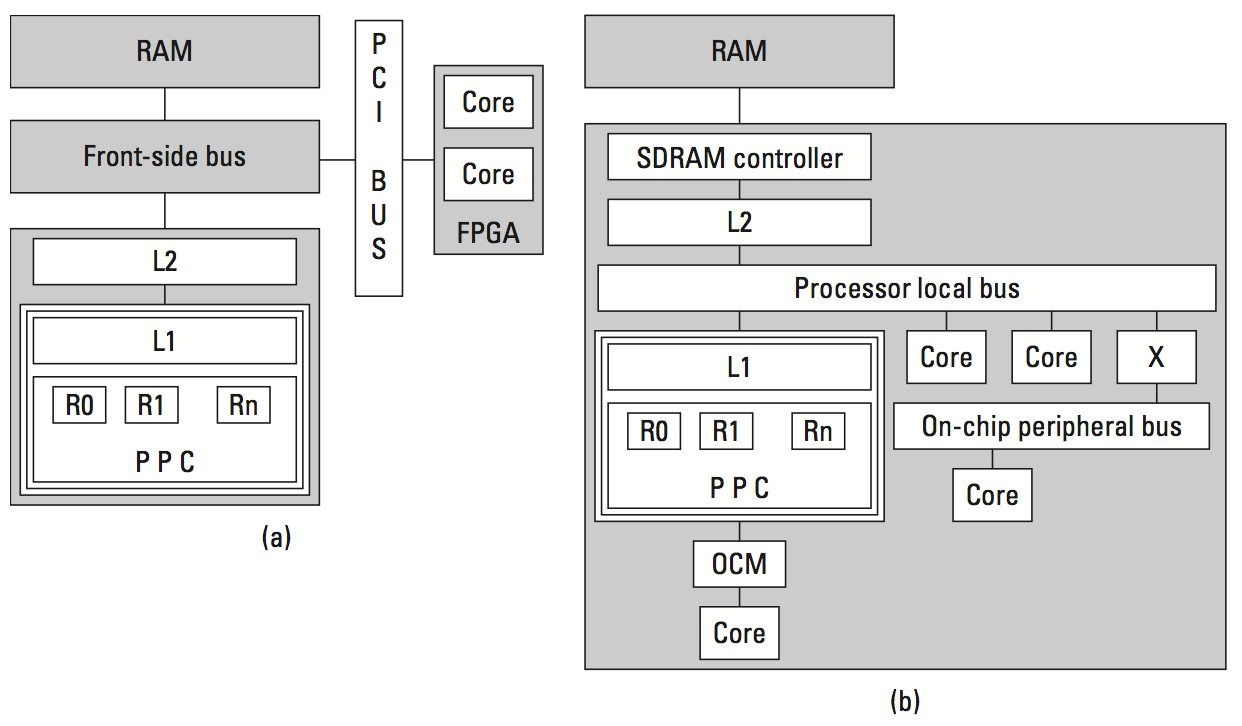
\includegraphics[width=1\textwidth]{img/f4-7.png}
			\caption{Situações na qual pode ocorrer bloqueio de estado. \textit{a)} Situação na qual existe um processador externo ao FPGA e sua memória interna é inacessível. \textit{b)} Situação onde o processador situa-se na plataforma FPGA. Fonte: \cite{Sass2010}.}
			\label{fig:4-7}
		\end{figure}

		Em ambos os casos mostrados na Figura \ref{fig:4-7} o FPGA (representado pelos \cores\ não possui autorização para o acesso aos registradores do processador (representados por $R_n$). Mesmo em \textit{b)} onde o processador é integrado à plataforma FPGA, não possui-se acesso sendo necessário a disponibilização manual deste.
	\end{description}


\subsection{Problema de Transferência de Estado}
	Estados afetados que estão presos necessitam de ser explicitamente comunicados e esta é feita por um processo chamado \textit{marshaling}.
    Assim, será feito um \textit{Marshaling} de grupos de elementos de um estado afetado de uma aplicação em registros lógicos que são explicitamente transferidos.

    Tendo a premissa que o processador possui o controle inicial, tem-se quatro tipos de registros que podem ser utilizados.
    Os dois primeiros, \textit{Type-I} e \textit{Type-F}, são utilizados para iniciar e outro para finalizar a transferência de um conjunto de elementos para o recurso, respectivamente.
    Os outros dois tipos de \textit{marshal} são usados repetidamente. Um quando o recurso é invocado (\textit{Type-CI}, do inglês \textit{copy-in}), e quando é completado (\textit{Type-CO}, do inglês \textit{copy-out}).
    %Um exemplo de \textit{Type-F} é quando tem-se um \core\ que acumula um valor em uma variável global. O registro \textit{Type-F} seria utilizado para ler o valor da variável após sua última invocação.

	Um processo de tradução pode ser incorporado com o \textit{marshaling}, sendo o exemplo a conversão de ponto flutuante para fixo quando transferido para um recurso o que acontece também com transformações mais complexas.
    %O agrupamento de elementos é lógico pelo fato do \textit{assembly} não significar estritamente que os elementos são copiados para uma memória de locação contínua.

	A forma mais simples de transferir estados é copiando os registros, parando o processador enquanto o recuso processa.
    Este é chamado de \textit{push} os dados no qual transmite o dado antes da transferência do controle. Ao final, realiza-se o \textit{pulls} dos dados.


    Embora simples uma transferência instantânea de estado não é sempre simples. Quando o estado afetado é grande mas o dado atua é pequeno, o padrão de acesso ao dado é randômico e a transferência lógica de registro é larga sendo mais vantajoso o uso de interfaces de comunicação para servir o recurso. Ou seja, utilizado quando o recurso foi designado para reduzir a latência da tarefa e a transferência do registo é pequena.
    Quando o registro lógico e o dado atual são largos, utiliza-se de padrão de acesso regula que transmite dados continuamente. É usado quando o recurso aumenta o \textit{throughput} e a redução de latência ou metas de performance não são possíveis.

    Isso é útil por exemplo na ordenação onde transferir um arranjo completo quando invocado é uma operação cara e desnecessária já que dependendo do algoritmo, pode-se utilizar apenas frações deste.

\end{comment}







\section{O Particionamento de \HS} \label{chap:desenvolvimento}

	%Para dar início ao problema, será considerado como aplicação um conjunto de instruções organizadas, como uma coleção de grafos de controle de fluxo especificando a sua ordem de execução.

	%Alguns fatores podem ajudar nas decisões de particionamento tal como expectativa de ganho de performance (Seção \ref{sec:performance}), os recursos utilizados em \hardware\ (Seção \ref{sec:recursos}), a forma na qual são usados e, talvez os mais importantes, quanto de sobrecarga de comunicação a decomposição impõe (Seção \ref{sec:comunicacao}) \todo{deixar?}e dificuldade de implementar um conjunto específico em \hardware\ (Seção \ref{sec:dificuldades}).

Algumas definições prévias:\todo[inline]{parei aqui}
	\begin{itemize}
    	\item \textbf{Recurso:} grupo conectado de instruções de uma aplicação de \design\ referencial de \software\ `adequado' para uma implementação em \hardware;

        O recurso pode variar de um pequeno conjunto de instruções até um modulo de \software\ completo consistente de múltiplas sub-rotinas. Como o tamanho dos recursos afetam na performance, a decisão de implementação em \hardware\ depende da sua melhoria no sistema por inteiro e mensura-se os recursos utilizados com relação a outros recursos candidatos.

        Se determinado que o recurso é vantagem, então os recursos de implementação em \hardware\ aumentam a arquitetura de \hardware.

        \item \textbf{Implementação em \hardware:} recurso adicional de uma específica aplicação;

        \item \textbf{Adequado:} descrevendo de forma mais geral no âmbito de sistemas embutidos, é a definição da situação na qual o projetista do sistema antecipa a percepção de vantagens na implementação em \hardware. %Para obter uma boa partição, geralmente deve-se examinar grupos que podem ser maiores ou menores que sub-rotinas definidas pelo programador.
    \end{itemize}

	\begin{figure}[!b] \centering
		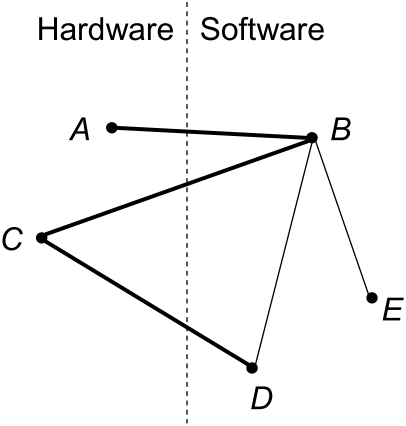
\includegraphics[width=0.18\textwidth]{img/partitioning.png}
		\caption{Representação Geral de um Particionamento em um grafo não direcionado. Os $\bullet$ (pontos) representam componentes da aplicação e as --- (linhas) seus respectivos fluxos de comunicação. A linha tracejada representa a divisão de níveis entre eles, sendo este \hs. Fonte: \cite{Mann2007}.}
		\label{fig:f4-4}
	\end{figure}

%\subsection{Declaração Formal do Problema}
%	Descreveremos problema segundo a definição de \cite{Arato2005, Mann2007} a seguir.

	%\subsection{Solução analítica para particionamento}
%\subsection{Visão Analítica Para o Particionamento}
\subsection{Declaração do Problema}
	Nesta seção será descrita as fórmulas matemáticas do problema de agrupamento de instruções em recursos e seus mapeamentos em \hardware\ ou \software.
	Segundo \cite{Sass2010}, a forma mais comum de transcrever é descrever manualmente o \core\ com um HDL utilizando \design\ referencial de \software\ como especificação, método utilizado para descrever o problema.

	No particionamento, muitos problemas práticos impactam diretamente na performance do sistema.
    Nem todos os problemas podem ser incorporados num modelo analítico \cite{Wang2016}, e por isso, só podemos esperar que as soluções matemáticas produzam uma uma resposta aproximada ao problema de particionamento ao utilizar a declaração formal.

	Muitas das entradas do modelo são estimadas ou aproximações no qual futuramente degrada a fidelidade de resultados.
    %Este é um fato relevante pois com isso, resolvendo o problema de particionamento `no papel', tem-se um particionamento que é próximo ao ótimo.
	%Assim, cabe ao \designer\ ser habilidoso em usar os guias e projetar uma solução mais refinada.
	Dessa forma, é mais eficiente usar uma combinação de técnicas \textit{ad hoc} e matemáticas para encontrar uma solução ótima ou aproximada do que simplesmente confiar numa intuição.


%\begin{comment}
%\subsection{Declaração do Problema}
	Já descrito as ferramentas matemáticas necessárias para descrever o problema fundamental do particionamento no Capítulo \ref{chap:revisao_bibliografica}, pode-se então, primeiramente, descrever formalmente o problema em termos de variáveis e descrever um algoritmo para encontrar uma solução aproximada.

		A ideia básica consiste em encontrar um particionamento para todos os blocos básicos de uma aplicação e então separá-los em \hs.
        Formalmente, procura-se por uma partição $ \mathcal{P} $ de todos os blocos básicos $ U $ de uma aplicação (Equação \ref{eq:bigcup})

        $$ U = \bigcup_{C \in \mathcal{C}} B(C) $$

		%$ C = (B,F) $
		Definida a partição e o universo, tem-se então um subconjunto $ \mathbb{C}\ |\ \mathbb{C} \subseteq U $, onde $ C \in \mathcal{C} $ é um vértice de um grafo de \design\ referencial de \software\ $ \mathcal{A} = (\mathcal{C}, \mathcal{L}) $ (oriundo da Equação \ref{eq:a}). O conjunto $ \mathbb{C} $, chamado conjunto de candidatos, contém todos os recursos arquiteturais potenciais, ou seja, o subconjunto de $ U $ que é esperado para melhorar a performance do sistema se implementado em um \hardware\ reconfigurável.
        Devido ao limite de recursos, deve-se refinar para o subconjunto $ \mathbb{D} \subseteq \mathbb{C} $ que maximiza nosso métrica de performance. Assim

		\begin{comment}
			\begin{eqnarray}
				\Gamma ( \mathbb{D}) \text{ é maximizado, e } \\
				\sum_{i \in \mathbb{d}} \vec{r}(i) < \vec{r}_{FPGA}
			\end{eqnarray}
		\end{comment}

		\begin{comment}
		\begin{table}[h]
			\begin{tabular}{rrcl}
			max                 & $\Gamma ( \mathbb{D})$               & ~   & ~                \\
			\textit{subject to} & $\sum_{i \in \mathbb{D}} \vec{r}(i)$ & $<$ & $\vec{r}_{FPGA}\label{eq:constraints}$
			\end{tabular}
		\end{table}
		\end{comment}

			\begin{equation}
					\begin{array}{rrcl}
					\text{max}                 & \Gamma ( \mathbb{D})               & ~   & ~                \\
					subject\ to & \sum_{i \in \mathbb{D}} \vec{r}(i) & < & \vec{r}_{FPGA}
					\end{array}
                    \label{eq:constraints}
			\end{equation}

		Algoritcamente, uma abordagem desse problema seria encontrar todas as partições de $ U $, sintetizando e \textit{profiling} cada partição, e então, quantitativamente avaliar cada $ \Gamma $. 
        %Como este é um problema linear inteiro (Seção \ref{sec:pli}) devido à alocação e utilização dos recurso físicos do FPGA, será escolhida uma abordagem heurística para tal \cite{Arato2003, Wang2016}.

\begin{comment}
\subsection{Abordagem Heurística}
	O problema de particionamento é essencialmente uma questão indireta de manipulação de parâmetros $ p(i) $ e $ \gamma(i) $ (tempo gasto em e ganho de performance, respectivamente) pelo rearranjo do particionamento $ \mathcal{X} $. Então seleciona-se os elementos de $ \mathcal{X} $ que satisfaz as restrições de recurso e maximiza a performance do sistema $ \Gamma $, Equação \ref{eq:constraints}.

	Uma metodologia heurística que pode ser aplicada informalmente é iniciar a partição natural provida pelo \design\ referencial de \software, ou seja, utiliza-se as sub-rotinas de uma aplicação original.

    Utilizando a ferramenta de \textit{profiling}, lista-se as sub-rotinas em ordem decrescente em tempo e verifica-se as que possuem maior valor $ p $. O valor de $ \gamma $ será estimado pela performance esperada a partir da implementação em \hardware\ e ao final, tem-se um ganho estimado do sistema para cada sub-rotina.

	Em seguida, quer-se manipular iterativamente a partição $ \mathcal{X} = \{ X_0, X_1, X_2, ...\} $ criando um novo subconjunto de blocos básicos por meio de operações de casamento e movimentações de blocos.
    A ideia em realizar alterações iterativas é encontrar mudanças que podem alterar os valores da fração $ p $ ou o valor de $ \gamma $.

    \begin{comment}
	\subsubsection{Fração do Tempo de Execução e Ganho de Performance} \label{sec:performance}
    \todo[inline]{Acho que esta parte do livro está errada}
		Uma forma de aumentar a fração de tempo gasta de uma sub-rotina, \todo{ou seja, diminuir seu tempo,} é torná-la maior na quantidade de recurso alocada a ela, por exemplo, casando vários blocos básicos num único bloco. Isso pode ser alcançado procurando por relações no grafo de chamadas ou, após a manipulação, por relacionamentos no grafo de controle de fluxo que conecta subconjuntos.

        Por exemplo, supondo que uma aplicação que teve seu tempo $ p(i) = 0,005 $ gaste:
        \begin{itemize}
        	\item $ 0,5\% $ numa sub-rotina \textit{A}; e
            \item $ 0,25\% $ nas sub-rotina \textit{B} e \textit{C}.
        \end{itemize}

        A fração de tempo gasto em \textit{A} pode ser duplicada pelo casamento de \textit{A, B} e \textit{C}. Entretanto, isso possui seu preço. Geralmente, aumenta-se o número de recursos utilizados e também pode aumentar no tamanho do subconjunto do sistema, decrescendo sua performance.
	\end{comme nt}

	\subsubsection{Ganho de Performance} \label{sec:performance}

		Para aumentar o ganho performance de recurso $ \gamma (i) $ necessita-se verificar o grafo de controle de fluxo do recurso e avaliar se uma mudança o tornará mais sequencial ou paralelo.

        Frequentemente, algoritmos que são inerentemente sequenciais, ou seja, uma forte dependência em seu fluxo ou dependências de controle, possuem melhor performance em processadores, por este não ter a sobrecarga de configurações de transistores e de possuírem melhor gerenciamento de energia nessas circunstâncias.
        Ou seja, simplesmente adicionar blocos básicos pode ter um efeito indesejável de aumentar o comportamento sequencial do recurso, reduzindo o valor de $ \gamma $.
        Entretanto, se um componente utilizar-se de menos recursos, então possui potencial de aumentar seu ganho de desempenho pela simplicidade. Exemplificando de uma forma mais geral, considara-se uma sub-rotina $ X $ e quebrando-a em duas sob-rotinas $ X – X' $ e $ X' $, onde a sub-rotina $ X – X' $ invoca $ X' $.
        Então se $ X' $ extrai partes de $ X $ que podem ser melhoradas em nível de \hardware\ deixando a parte sequencial em $ X – X' $, então $ \gamma $ de $ X' $ será maior que $ \gamma $ de $ X $ original e provavelmente necessitará de menos recursos.

        %Assim, supondo uma sub-rotina tome $ 93\% $ de tempo e provê um ganho de $ \gamma = 2 $, então a aplicação terá performance de $ \Gamma = 1.869 $. Entretanto, se uma parte da sub-rotina pode ser extraída aumentando o paralelismo, então é possível que a performance poderia aumentar em dez vezes tendo o $ \gamma = 20 $ e com isso, o tempo decrescendo para $ 83\% $. Esse particionamento gera um \speedup\ de $ \Gamma = 4.739 $.

		%A lei de Ahmdal tenta sempre aumentar a fração de tempo gasto na porção de código que acaba de ser melhorada.
        %No entanto, quando limitado os recursos, nem sempre é melhor.

		Com isso é importante notar que qualquer mudança no subconjunto pode afetar a performance para melhor ou pior.
        Em geral, heurísticas trabalham examinando os grafos da aplicação e então fazendo mudanças incrementais ao subconjunto de uma partição.
        Tais mudanças são guiadas pela tentativa de diminuir o tempo gasto em uma sub-rotina não aumentando dramaticamente seus recursos ou decrescendo sua performance; e a tentativa de aumentar a performance sem aumentar o tempo gasto em uma sub-rotina.


\begin{comment}
\subsection{\Benchmarks}
	\cite{Trindade2016}

	% intro
	Por serem um excelente mensurador de performance de aplicações e processadores, \designs\ têm feito de \benchmarks\ uma parte crítica do processo de \design\ de projetos.
	Uma vez que um \benchmark\ torna-se padrão e popular em um ramo de pesquisa, cria-se então uma alta pressão em aumento de performance por otimizações \cite{Hennessy2011}.

	% utilização de benchs no trabalho
	% arato2005
	Para a demonstração e validação da solução a ser desenvolvida, será utilizado %vários \benchmarks\ e exemplos randômicos largos.
	\benchmark\ de \textit{MiBench}.
	Esse \benchmark, segundo \cite{Guthaus2001} foi escolhido com base em um exame e comparação de um conjunto de aplicações embarcadas representativas comercialmente com o conjunto de \benchmarks\ SPEC2000 \cite{Case1995}.
\end{comment}

\section{Resultados}



Lorem ipsum dolor sit amet, consectetur adipiscing elit. Donec convallis lorem et felis feugiat, non accumsan nibh vehicula. Duis venenatis, turpis et tincidunt pretium, lacus mauris facilisis turpis, vitae aliquet dolor mauris nec sapien. Mauris laoreet quam nisl, sit amet cursus libero elementum et. Curabitur dolor arcu, scelerisque sit amet est in, suscipit ornare nibh. Maecenas et nunc condimentum, tincidunt velit eget, sagittis enim. Interdum et malesuada fames ac ante ipsum primis in faucibus. Nulla posuere nisi non dolor cursus, id dignissim dolor fringilla.

Proin pulvinar, dui in pharetra fermentum, diam ipsum commodo nunc, accumsan porttitor nulla nisl sed erat. Proin quis nibh id purus aliquet sodales in quis libero. Duis id sem hendrerit, faucibus nibh nec, volutpat felis. Curabitur sollicitudin risus vel orci ultricies, ut rhoncus lorem vehicula. Curabitur ultricies volutpat arcu, quis interdum ex venenatis eget. Praesent volutpat euismod vehicula. Fusce fermentum mauris mauris, vel commodo dui ornare eu. Nam dapibus vestibulum quam quis molestie. Interdum et malesuada fames ac ante ipsum primis in faucibus. Donec vitae ornare ex. Aliquam erat volutpat. Class aptent taciti sociosqu ad litora torquent per conubia nostra, per inceptos himenaeos. Vestibulum sollicitudin euismod orci, sed venenatis lectus laoreet aliquet. Vestibulum vehicula lectus neque, et lacinia neque tincidunt et.

Cras porttitor sem sed purus iaculis, ac finibus nisl laoreet. Proin efficitur, est et convallis consequat, arcu nulla elementum elit, eu ultrices massa libero eget justo. Morbi pretium neque nec ultrices venenatis. Vivamus ac bibendum justo, sit amet posuere risus. Proin sodales non libero at varius. Nunc nec turpis ante. Sed condimentum leo est, ac consectetur nunc cursus nec. Cras quis metus tempor erat varius iaculis vitae eget nunc. Duis non libero quis sem bibendum tempor. Aenean dolor purus, mattis in diam at, ullamcorper mattis dui. Suspendisse eget enim luctus, dapibus nisl faucibus, condimentum lacus. Sed vitae cursus nibh. Pellentesque habitant morbi tristique senectus et netus et malesuada fames ac turpis egestas. Donec gravida erat id lectus maximus, a eleifend massa convallis. Sed porttitor maximus consectetur. Mauris congue porta leo quis elementum.

Cras non elit eu sapien commodo cursus nec id massa. Nullam consequat pharetra lacus, sit amet faucibus neque congue facilisis. Aliquam accumsan vel eros eu consectetur. Quisque est ligula, maximus ac lacus eu, mollis faucibus massa. Aliquam quis nisi ac mi sagittis scelerisque non vitae nisl. Ut vitae velit purus. Quisque vel aliquam urna, sit amet maximus est. Suspendisse potenti. Curabitur faucibus molestie nibh. Sed feugiat pellentesque odio, et scelerisque nibh semper et. Morbi congue venenatis odio sit amet auctor. Suspendisse scelerisque aliquet fringilla. Quisque eu auctor nulla. Vestibulum porta lacus eget iaculis commodo.

Nam vestibulum eleifend mauris sed tempor. Nulla tellus nisl, consectetur eu mauris vel, vulputate malesuada lacus. Aenean eget lectus purus. Vestibulum eget augue nisi. Ut auctor neque vel mauris rutrum, eget bibendum nisi convallis. Fusce sagittis egestas magna. Nullam gravida nec dui et accumsan. Aenean luctus quis libero mollis tincidunt. Etiam varius ligula sed ante interdum, at egestas nisi tempus. Etiam in tellus et mi interdum elementum vel et turpis. Curabitur vulputate orci quam, ut interdum massa vehicula id. Fusce viverra orci non lorem ornare accumsan. Nulla commodo nunc dui, sit amet bibendum nunc tincidunt quis. Sed mollis feugiat nisl, id placerat nisl molestie in.

Morbi sagittis nisl arcu, ut interdum urna egestas id. Nulla quis sollicitudin ante, a vulputate mi. Nullam efficitur aliquet purus, non ultricies leo sagittis id. Donec in dignissim mauris. Pellentesque tempus eget ante et tincidunt. In nec diam eros. Donec pretium orci vitae nisl congue condimentum. Cras feugiat vel ex id iaculis. Maecenas condimentum efficitur imperdiet.

Phasellus imperdiet, justo gravida scelerisque elementum, ligula enim iaculis massa, in placerat purus massa in nisi. Nulla vel sem orci. Etiam ultricies nulla a dui lobortis, non vehicula magna molestie. Nulla vel mattis nibh. Mauris sed porta nibh, eget aliquam orci. Nam sit amet ipsum est. Quisque orci est, vehicula et elit ut, ultrices efficitur leo. Nam sollicitudin, dolor vel facilisis aliquet, felis metus mattis lacus, ut interdum eros erat a lorem. Nulla facilisi. Maecenas accumsan dolor ut felis dictum aliquam. Suspendisse ac arcu suscipit, luctus dolor et, lobortis lectus. Cras ut turpis nec dolor iaculis malesuada in et purus. Cras turpis velit, imperdiet nec posuere nec, efficitur et ipsum. Sed aliquam, dolor tristique elementum venenatis, quam justo tincidunt dolor, nec porttitor elit ipsum sit amet lectus. Aenean et malesuada urna, vel rhoncus arcu. Maecenas ultricies vestibulum augue, nec egestas lectus luctus nec.

Curabitur id ex nec ligula varius placerat. Morbi laoreet augue sapien, et mattis nisl scelerisque ac. Pellentesque nec facilisis odio, eu fringilla risus. Etiam venenatis ex ut sem lacinia interdum. Phasellus laoreet porta augue, sit amet tempor est porttitor ut. Vestibulum purus dolor, finibus at dapibus vitae, mattis vel felis. Sed sagittis fermentum felis eget aliquam. Aliquam pharetra, mi id sollicitudin dignissim, orci tortor eleifend ante, a ultricies leo nisl sit amet purus. Lorem ipsum dolor sit amet, consectetur adipiscing elit.

Donec et cursus dui, ut aliquam lacus. Etiam mi sem, accumsan non consectetur et, mollis vel erat. Morbi venenatis ut eros nec sollicitudin. Nam semper, mauris vitae sagittis porta, est libero semper tortor, posuere volutpat mauris odio vitae libero. Nam facilisis ullamcorper mi. Vivamus lectus ante, rhoncus id tellus eu, iaculis vestibulum erat. Cras quis tortor consectetur, facilisis tortor aliquam, rhoncus mauris.

Vestibulum sollicitudin sagittis posuere. Aenean rutrum ante ut ultrices ullamcorper. Sed consequat quis est eu aliquet. Aenean ultrices interdum pulvinar. Fusce iaculis enim vel sapien congue commodo. Proin dictum lectus a sem posuere commodo. Praesent id risus convallis, molestie orci ac, vestibulum felis. Donec scelerisque sem turpis, nec pharetra lectus pellentesque vehicula. Quisque laoreet tempus felis id hendrerit. Duis venenatis a mauris a euismod. Nulla sapien mi, rhoncus a tincidunt in, vehicula id urna. Cras interdum, nibh eget dictum mollis, dui ante dictum nisl, ac aliquet diam quam sit amet ex. 
\begin{comment}
\begin{figure*}[!t]
\centering
\subfloat[Case I]{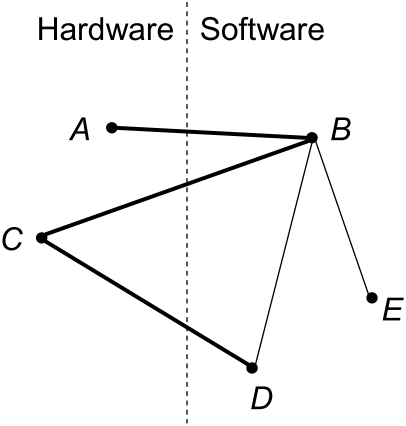
\includegraphics[width=2.5in]{img/partitioning.png}%
\label{fig_first_case}}
\hfil
\subfloat[Case II]{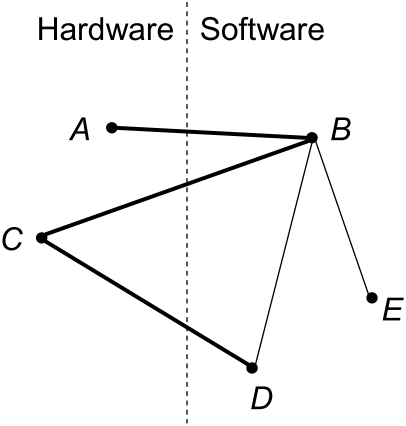
\includegraphics[width=2.5in]{img/partitioning.png}%
\label{img/fig_second_case}}
\caption{Simulation results for the network.}
\label{fig_sim}
\end{figure*}
\end{comment}


\section{Conclusion}
Lorem ipsum dolor sit amet, consectetur adipiscing elit. Cras tristique metus eget sem lobortis, vitae dapibus orci aliquam. Aenean aliquet, tellus eu eleifend consequat, erat metus rhoncus enim, vel fermentum lectus quam et neque. Proin urna ipsum, sodales facilisis tristique eget, vehicula id neque. Sed tristique augue vel ipsum ornare malesuada. Etiam blandit justo et mi ullamcorper, vitae molestie tortor sollicitudin. Phasellus id odio venenatis dui feugiat tristique vitae in augue. Aliquam lacus erat, semper in erat vel, aliquet tempus mauris. Mauris posuere dolor non eros ullamcorper lobortis. Mauris ut efficitur orci, sed cursus felis. Cras scelerisque tellus ut tempor egestas. 

Lorem ipsum dolor sit amet, consectetur adipiscing elit. Cras tristique metus eget sem lobortis, vitae dapibus orci aliquam. Aenean aliquet, tellus eu eleifend consequat, erat metus rhoncus enim, vel fermentum lectus quam et neque. Proin urna ipsum, sodales facilisis tristique eget, vehicula id neque. Sed tristique augue vel ipsum ornare malesuada. Etiam blandit justo et mi ullamcorper, vitae molestie tortor sollicitudin. Phasellus id odio venenatis dui feugiat tristique vitae in augue. Aliquam lacus erat, semper in erat vel, aliquet tempus mauris. Mauris posuere dolor non eros ullamcorper lobortis. Mauris ut efficitur orci, sed cursus felis. Cras scelerisque tellus ut tempor egestas. 

Donec et cursus dui, ut aliquam lacus. Etiam mi sem, accumsan non consectetur et, mollis vel erat. Morbi venenatis ut eros nec sollicitudin. Nam semper, mauris vitae sagittis porta, est libero semper tortor, posuere volutpat mauris odio vitae libero. Nam facilisis ullamcorper mi. Vivamus lectus ante, rhoncus id tellus eu, iaculis vestibulum erat. Cras quis tortor consectetur, facilisis tortor aliquam, rhoncus mauris.


% use section* for acknowledgment
\ifCLASSOPTIONcompsoc
  % The Computer Society usually uses the plural form
  \section*{Acknowledgments}
\else
  % regular IEEE prefers the singular form
  \section*{Acknowledgment}
\fi


Lorem ipsum dolor sit amet, consectetur adipiscing elit. Cras tristique metus eget sem lobortis, vitae dapibus orci aliquam. Aenean aliquet, tellus eu eleifend consequat, erat metus rhoncus enim, vel fermentum lectus quam et neque. Proin urna ipsum, sodales facilisis tristique eget, vehicula id neque.





% trigger a \newpage just before the given reference
% number - used to balance the columns on the last page
% adjust value as needed - may need to be readjusted if
% the document is modified later
%\IEEEtriggeratref{8}
% The "triggered" command can be changed if desired:
%\IEEEtriggercmd{\enlargethispage{-5in}}

\bibliographystyle{IEEEtran}
\bibliography{Mendeley}


% that's all folks
\end{document}
